\section{Specific requirements}

\subsection{External Interfaces}

\subsubsection{User Interface}
This section of the document illustrates the platform's user interfaces, graphical tools that facilitate users' interaction with the software.
\newline
Within the platform, there are two different types of views based on user roles: the Student and the Educator. Each role offers specific and distinct functionalities.
\newline
The Educator, can create and manage tournaments and battles. The Student, on the other hand, is able to actively participate in tournaments and battles.
\newline
This distinction of roles results in a differentiated user interface, specially designed to offer specific functionalities according to the profile and actions allowed to each type of user.
\vspace{0.5\baselineskip}

\begin{figure}[h]
    \centering
    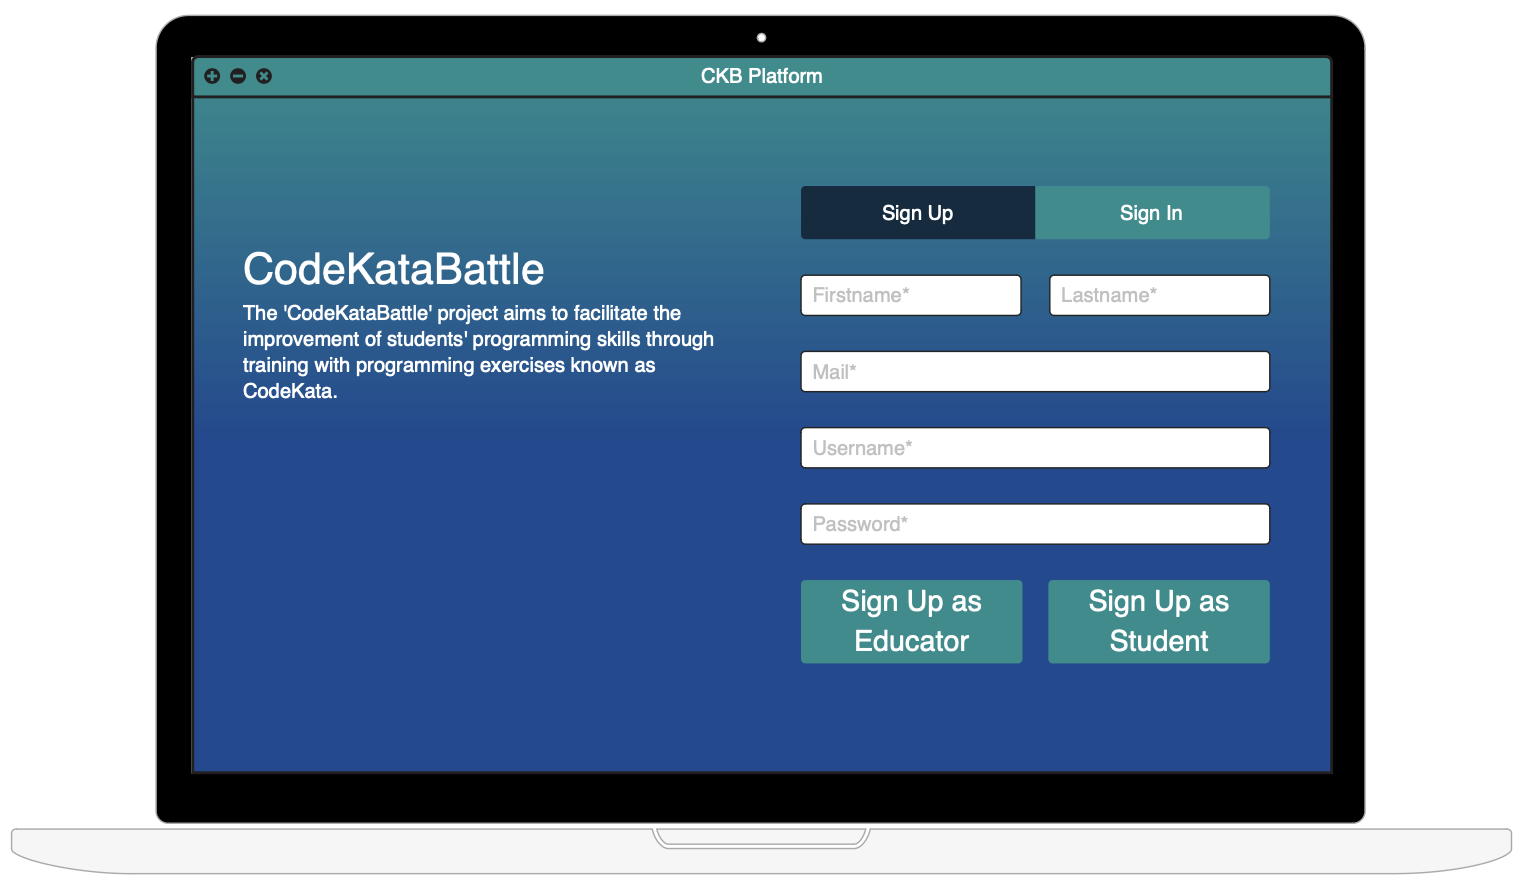
\includegraphics[scale=0.45]{images/Mockup/SignUpMockup.png} 
    \caption{User Interface to register on the platform}
    \label{fig_SignUpMockup}
\end{figure}

The figure \ref{fig_SignUpMockup} shows the user interface relating to the platform registration procedure. This interface allows users to enter their personal data, such as firstname, lastname and e-mail address, as well as provide a username and password to access the system. 
It also offers the possibility to select the desired type of registration, allowing users to register as a student or as an educator.

\vspace{0.5\baselineskip}
\clearpage

\begin{figure}[h]
    \centering
    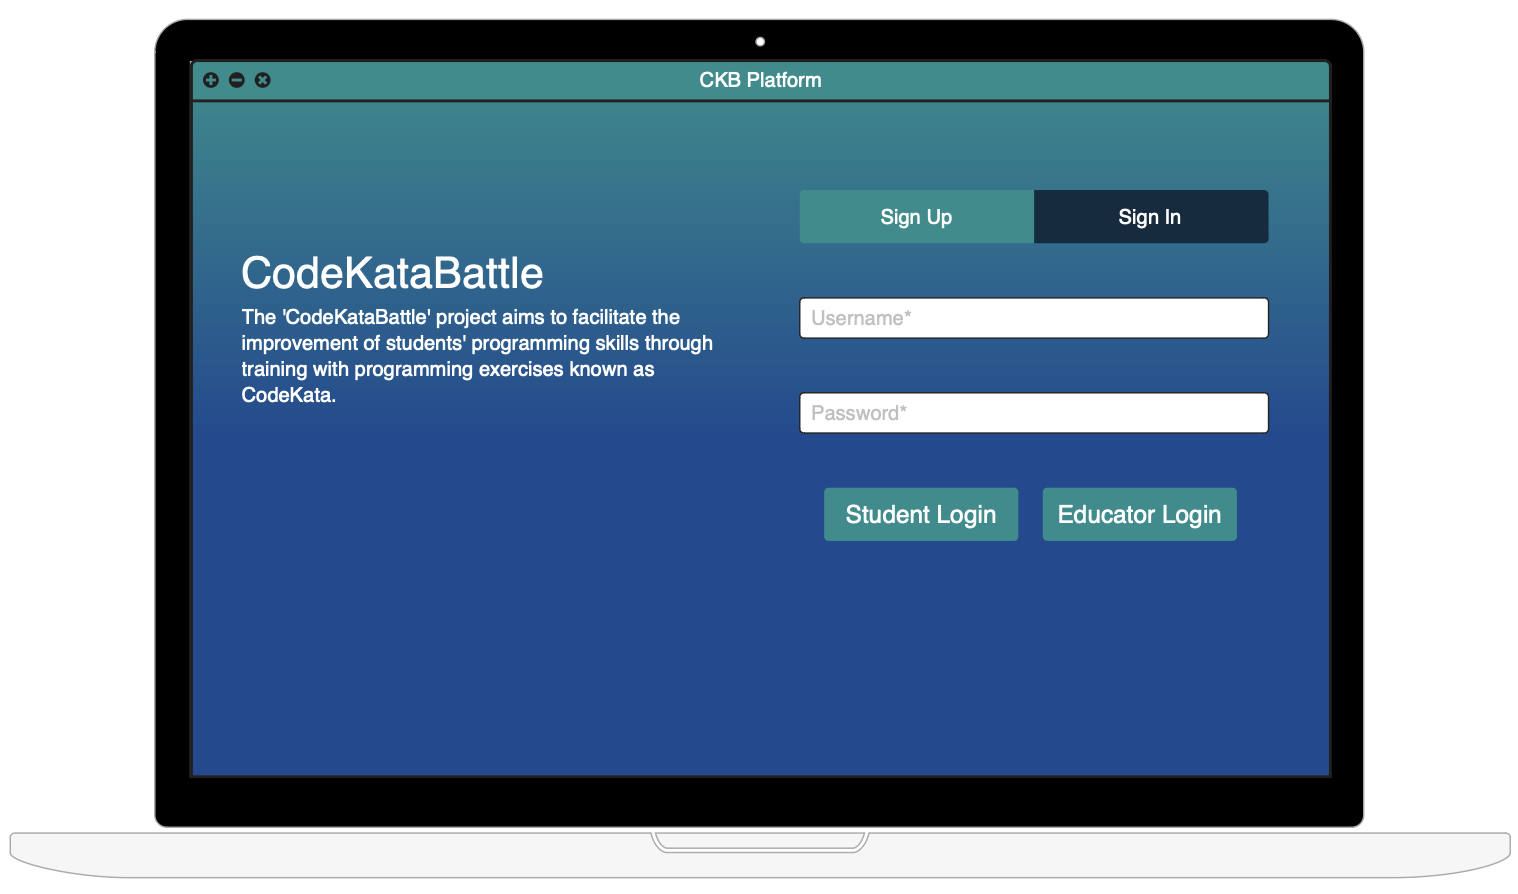
\includegraphics[scale=0.4]{images/Mockup/SignInMockup.png} 
    \caption{User Interface to login on the platform}
    \label{fig_SignInMockup}
\end{figure}

Figure \ref{fig_SignInMockup} illustrates the interface dedicated to accessing the platform. This screen allows users to enter their login credentials, including username and password. It also offers the choice of logging in as Educator or Student.

\vspace{0.5\baselineskip}
\begin{figure}[h]
    \centering
    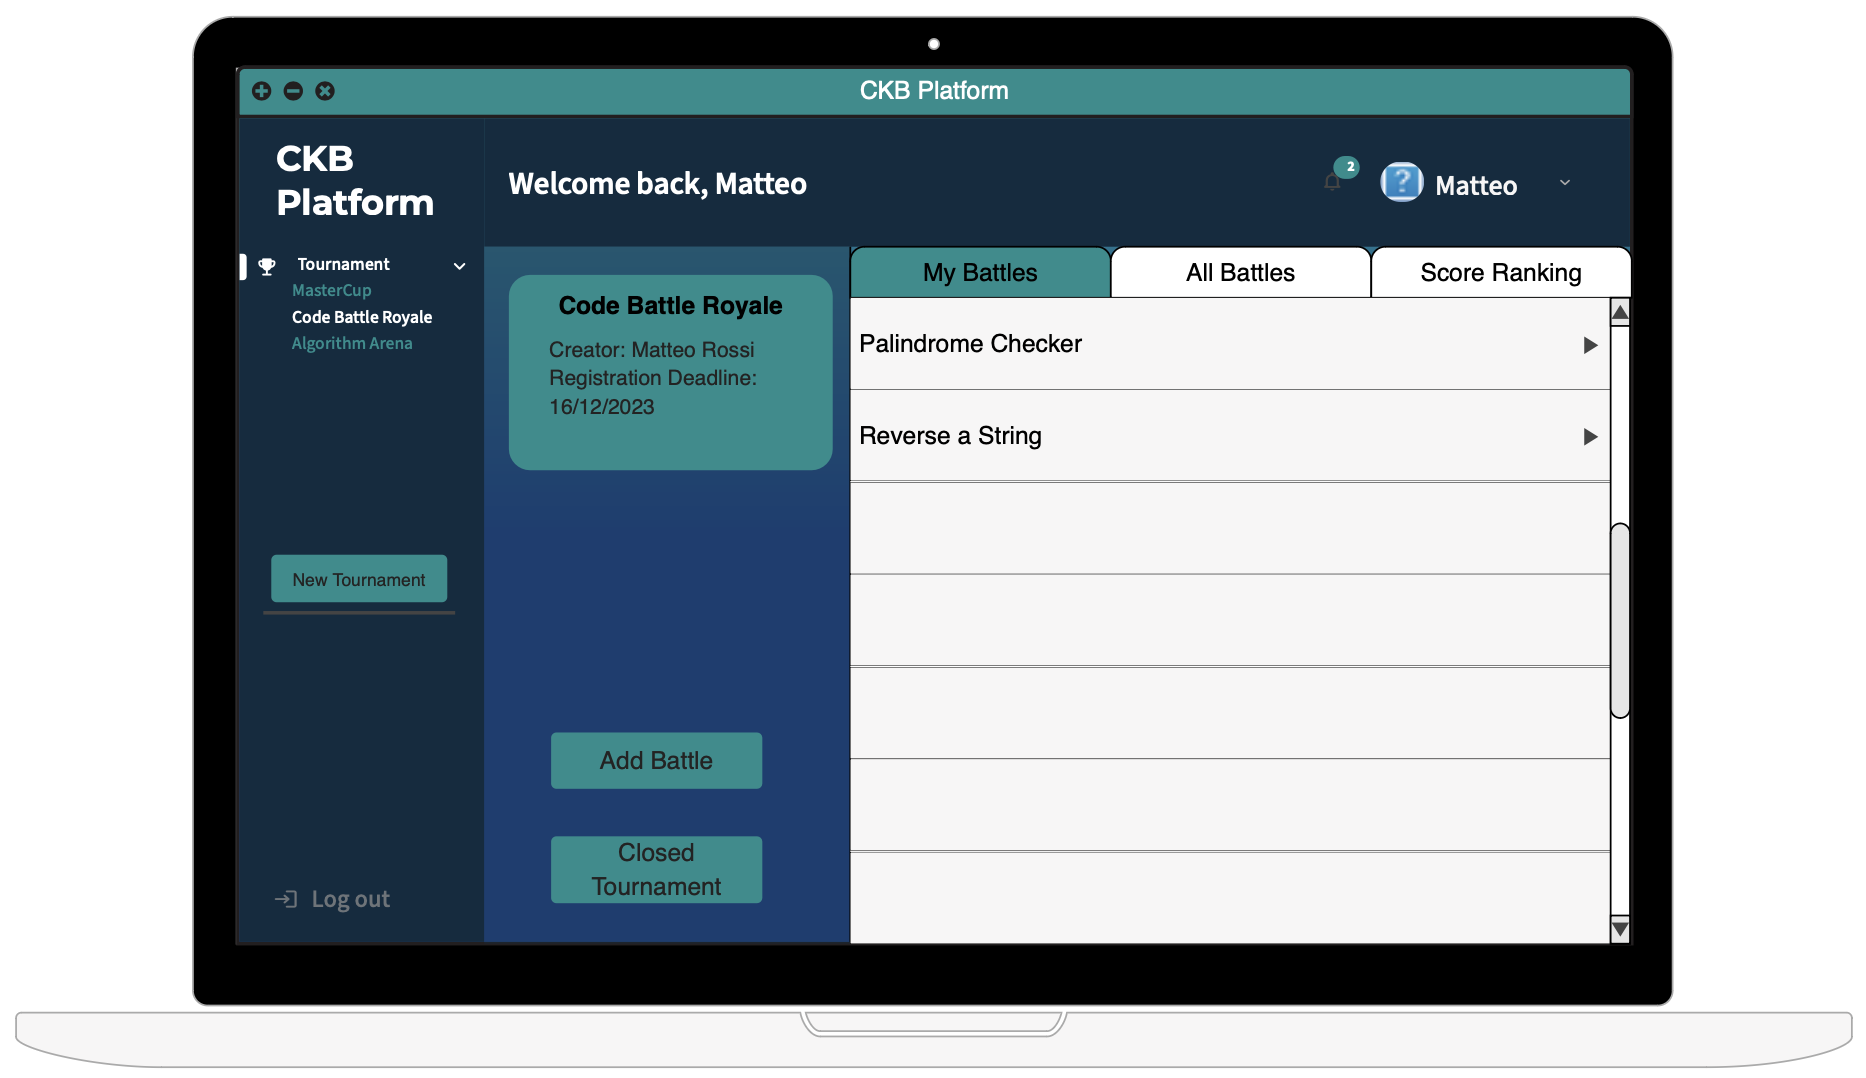
\includegraphics[scale=0.35]{images/Mockup/TournamentManageMockup.png} 
    \caption{Educator Interface for Tournament Management}
    \label{fig_TournamentManageMockup}
\end{figure}

Figure \ref{fig_TournamentManageMockup} represents the educator's interface for managing tournaments and related battles.
\newline
In the left section of the interface, a list of tournaments the educator is a creator of or participates in is displayed, as well as a 'New Tournament' button to create a new tournament.
\newline
Each tournament is accompanied by a descriptive section containing information such as the name of the tournament, the creator and the registration deadline .
In addition there are two buttons: 
\begin{itemize}
    \setlength{\itemsep}{0pt}
    \setlength{\parskip}{0pt}
    \setlength{\parsep}{0pt}
    \setlength{\partopsep}{0pt}
    \setlength{\topsep}{0pt}
    \item "Add Battle": allows the addition of new battles within the tournament.
    \item "Closed Tournament": allows to close the tournament only to the educator who created the tournament and if all battles have been completed.
\end{itemize}

The section to the right of the interface presents a series of selectable tabs that allow various information to be displayed:
\begin{itemize}
    \setlength{\itemsep}{0pt}
    \setlength{\parskip}{0pt}
    \setlength{\parsep}{0pt}
    \setlength{\partopsep}{0pt}
    \setlength{\topsep}{0pt}
    \item "My Battles": shows all battles created for that specific tournament by the educator.
    \item "All Battles": shows the complete list of all battles in the tournament.
    \item "Score Ranking: displays the ranking based on the scores of all those participating in the tournament.
\end{itemize}


\vspace{0.5\baselineskip}
\begin{figure}[h]
    \centering
    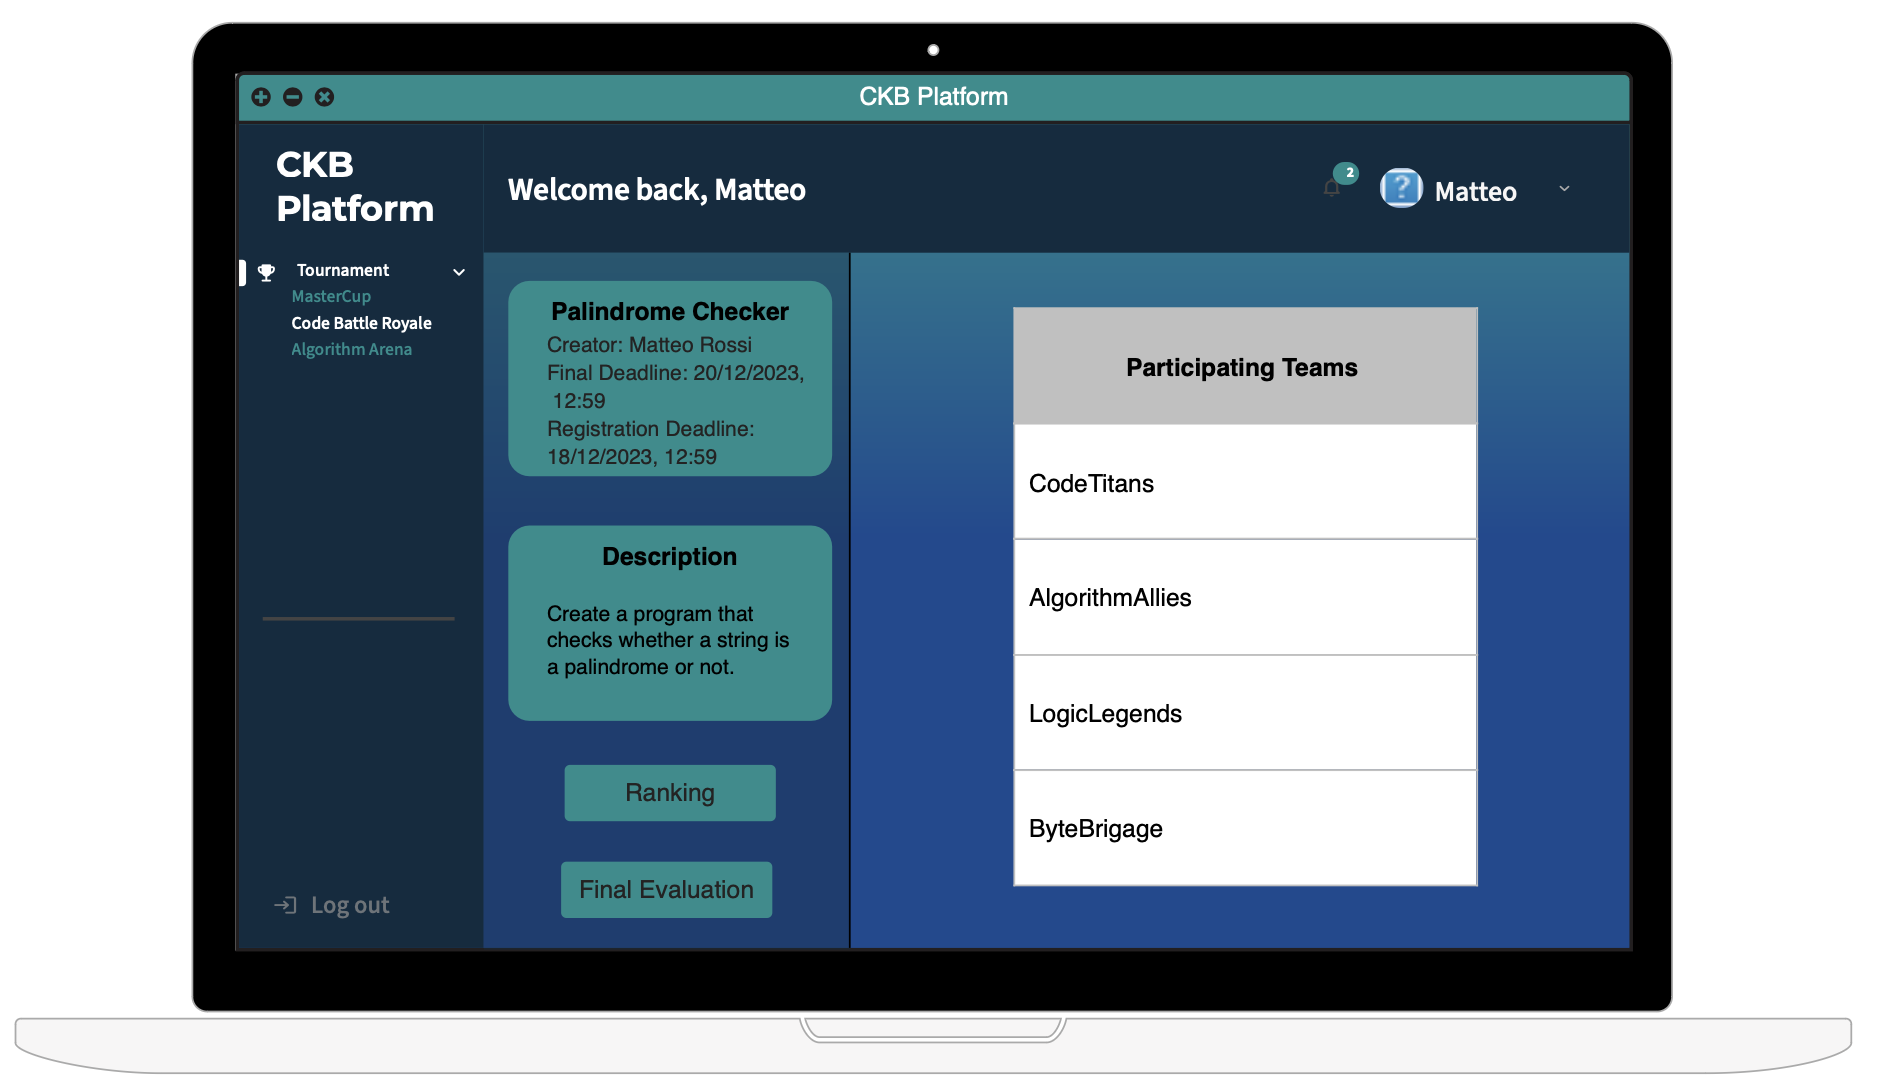
\includegraphics[scale=0.35]{images/Mockup/ListTeamsMockup.png} 
    \caption{Educator Interface for Battle Management}
    \label{fig_ListTeamsMockup}
\end{figure}

Once the battle has been selected, Figure \ref{fig_ListTeamsMockup} presents the interface dedicated to its management by the educator who is its creator.
\newline
In the left section of the interface, there are two containers. The first contains key information regarding the battle, including details such as the name, creator educator, final deadline and registration deadline. The second container contains a detailed description of the battle.
\newline
In addition, two buttons are available:
\begin{itemize}
    \setlength{\itemsep}{0pt}
    \setlength{\parskip}{0pt}
    \setlength{\parsep}{0pt}
    \setlength{\partopsep}{0pt}
    \setlength{\topsep}{0pt}
    \item "Ranking": displays the ranking for the battle.
    \item "Final Evaluation": only accessible if the battle is over, defined by the Final Deadline. It provides access to a dedicated screen to view the last source uploaded by each team and evaluate it..
\end{itemize}


In addition, the list of teams actively participating in the battle is presented in the right section of the interface.

\clearpage
\begin{figure}[h]
    \centering
    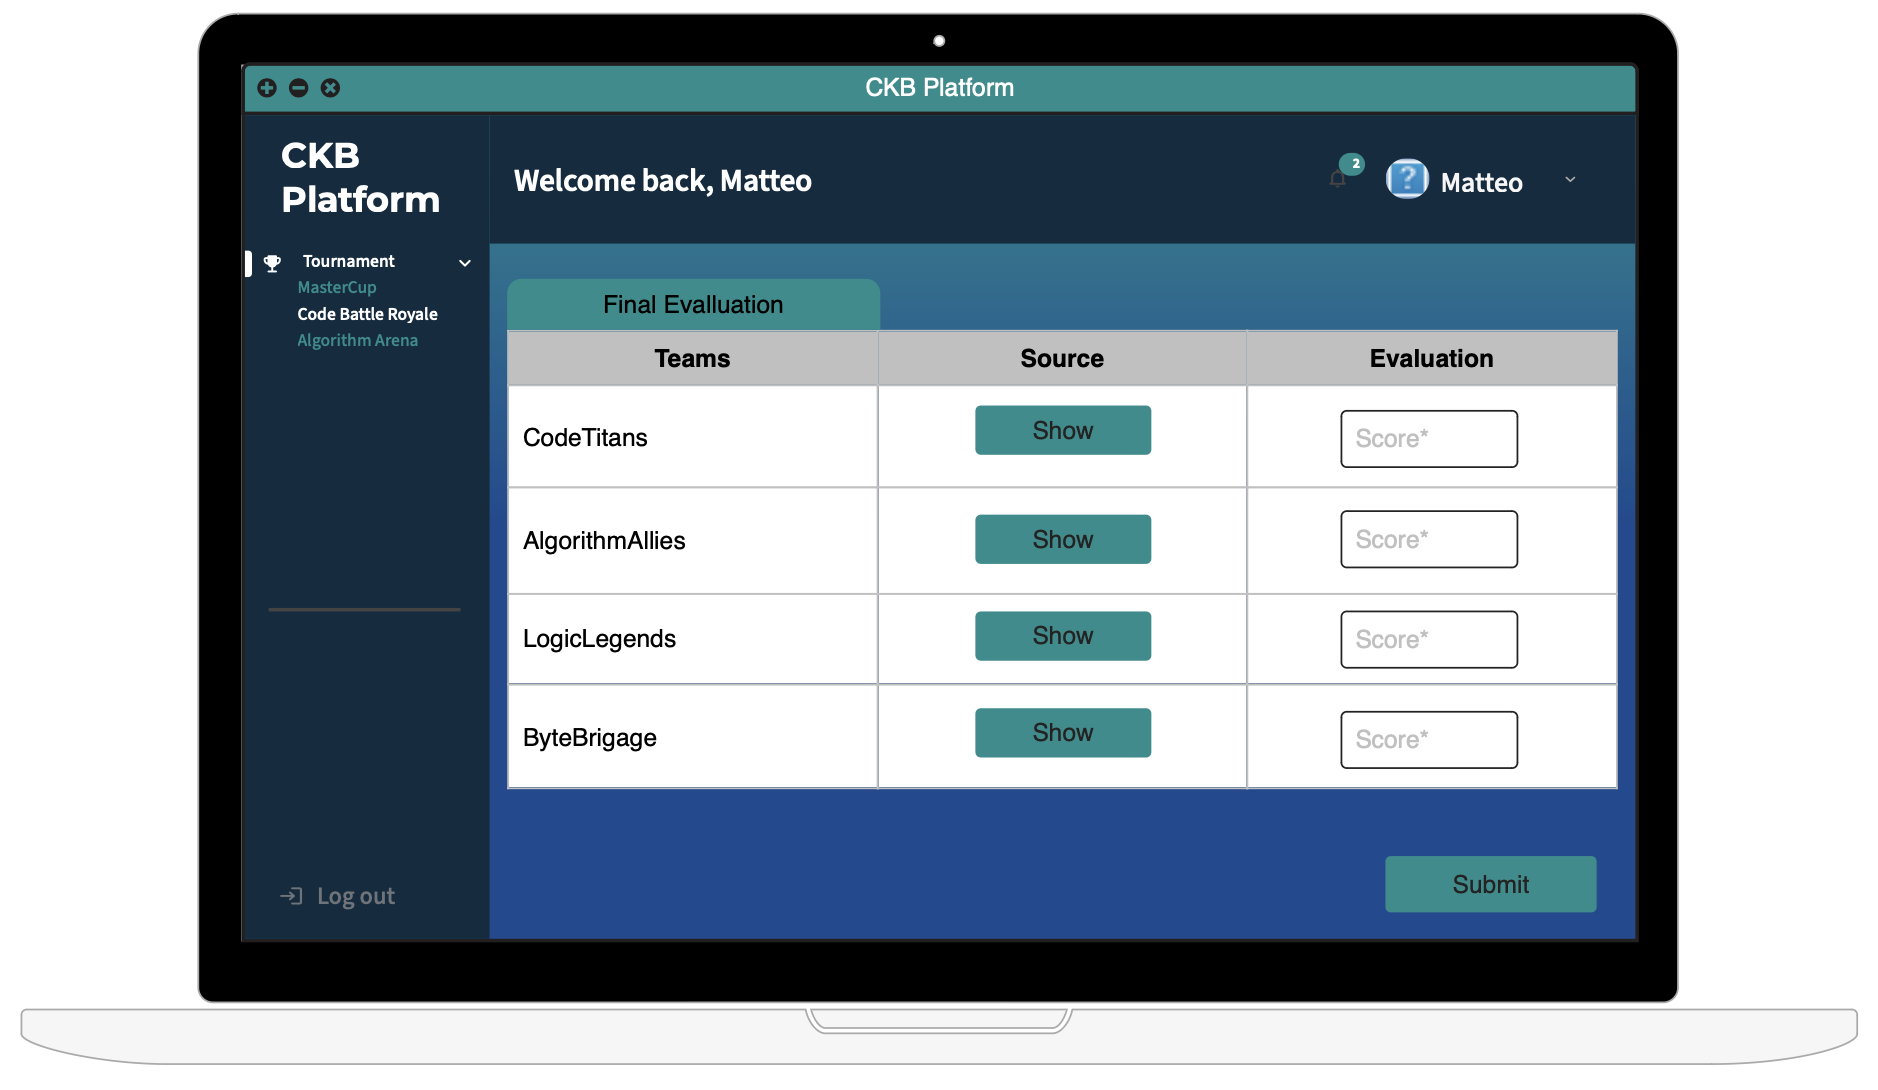
\includegraphics[scale=0.35]{images/Mockup/FinalEvaluationMockup.png} 
    \caption{Educator Interface for Final Evaluation}
    \label{fig_FinalEvaluationMockup}
\end{figure}
At the end of the battle, defined by the final deadline date, when the educator presses the 'Final Evaluation' button, he is shown the page in the Figure \ref{fig_FinalEvaluationMockup}. 
\newline
This section lists the participating teams with a corresponding button to access the source file. In addition, there is also a dedicated scoring section, which allows you to manually enter the value to be assigned to each team.
\newline
Once the scoring is completed, the operation is confirmed by pressing the 'Submit' button.


\begin{figure}[h]
    \centering
    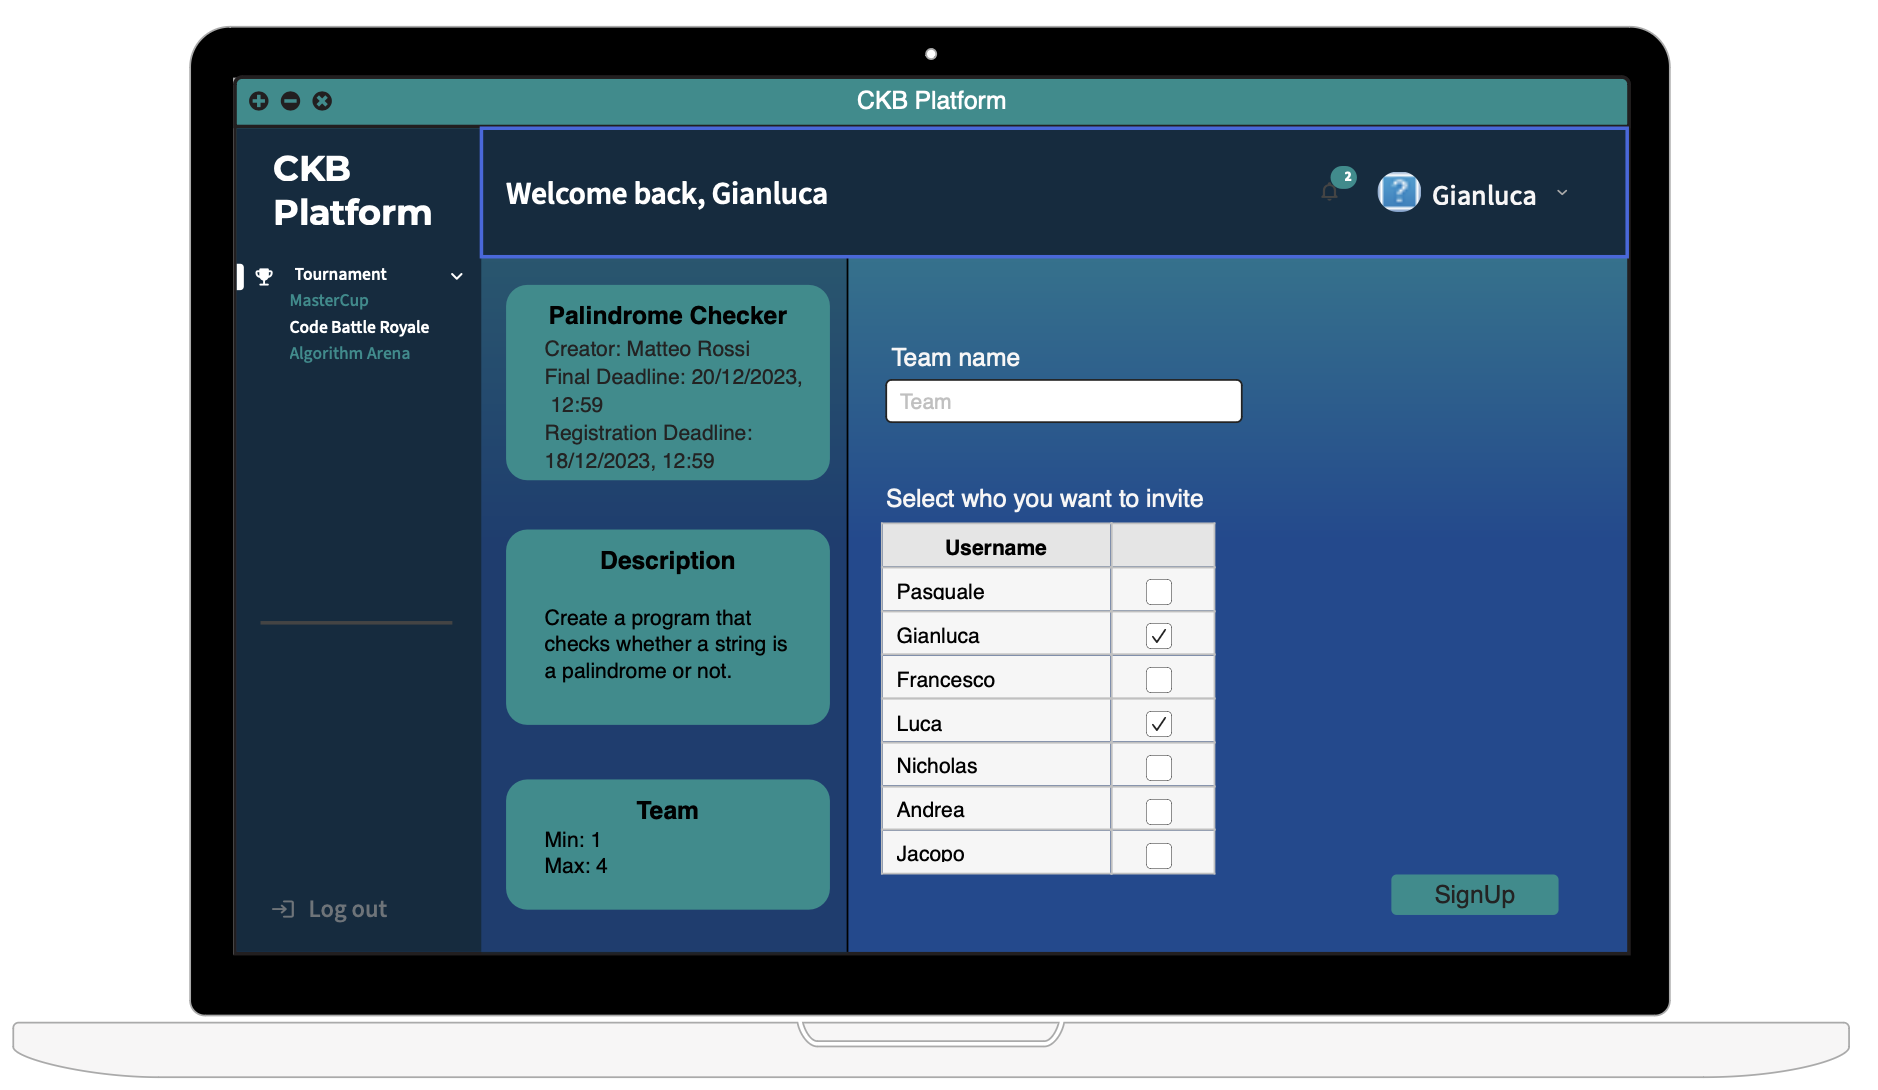
\includegraphics[scale=0.35]{images/Mockup/SignUpBattleMockup.png} 
    \caption{Student Interface to register for a battle}
    \label{fig_SignUpBattleMockup}
\end{figure}

Figure \ref{fig_SignUpBattleMockup} shows the interface that offers students the opportunity to register for a specific battle.  This screen allows students to form a team, entering the team name and inviting other students to the tournament, always respecting the limits set for the tournament itself, which are detailed in the dedicated section on the left of the interface.

\clearpage
\begin{figure}[h]
    \centering
    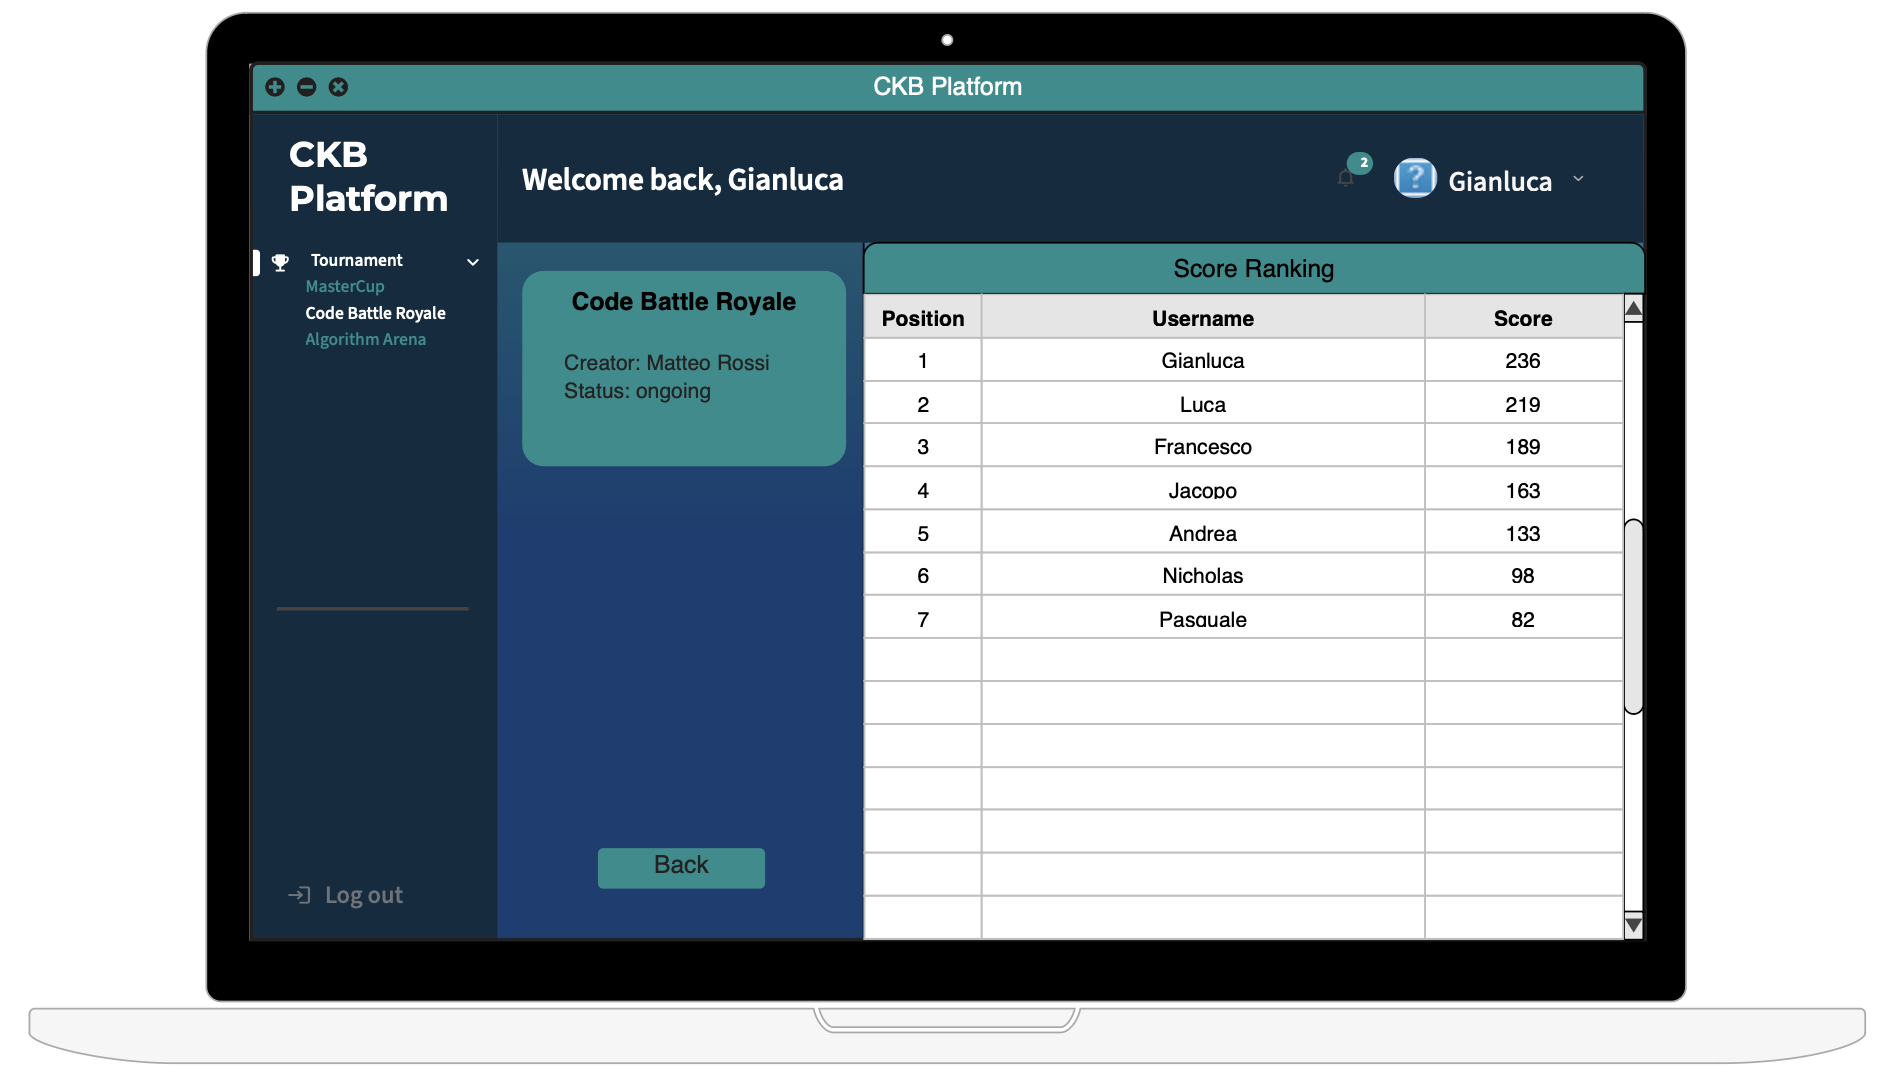
\includegraphics[scale=0.35]{images/Mockup/TournamentRankingMockup.png} 
    \caption{Interface for the Tournament Ranking}
    \label{fig_TournamentRankingMockup}
\end{figure}

The interface illustrated in Figure \ref{fig_TournamentRankingMockup} shows the detailed ranking of the tournament entrants, together with their respective scores, accessible to all registered members of the platform.
In addition, there is a button in the left section that allows you to return to the battle list





\subsubsection{Hardware interfaces}
The CKB system has no external hardware equipment to interact with.

\subsubsection{Software interfaces}
The system requires certain software interfaces in order to provide specific services. These interfaces are detailed below:
\begin{itemize}
    \item \textbf{GitHub REST API v3}: the system uses these APIs to enable communication with the GitHub platform and the execution of specific actions. Such actions include, for example, creating folders and performing pull operations related to specific directories.

    \item \textbf{SonarQube Web API}: these APIs make it possible to automate various operations, including the ability to upload projects and perform static analysis in accordance with specified parameters.
\end{itemize}

\subsubsection{Communication interfaces}
The system uses the Internet connection to communicate with all connected devices.
The backend of the system will expose a unified RESTful API to communicate with all clients using HTTPS and TCP/IP.
\clearpage

\subsection{Functional requirements}
Following are all the functional requirements divided by functionality.
\newline

\textbf{Registration and login requirements }

\begin{tabular}{|c|p{13.2cm}|}
  \hline
  \textbf{Rn} & \textbf{Description} \\
  \hline
  R1 & The system allows the student to register by entering firstname, lastname, email, username and password. \\
  \hline
  R2 & The system allows registered students to log in by entering username and password.  \\
  \hline
  R3 & The system allows the educator to register by entering firstname, lastname, email, password and username. \\
  \hline
  R4 & The system allows registered educator to log in by entering username and password. \\
  \hline
\end{tabular}

\clearpage
\textbf{Tournament requirements}

\begin{tabular}{|c|p{13.2cm}|}
  \hline
  \textbf{Rn} & \textbf{Description} \\
  \hline
  R5 & The system allows the educator the ability to create of a tournament, allowing him or her to set a deadline for entries. \\
  \hline
  R6 & The system allows the educator to invite other educators to join the tournament.   \\  
  \hline
  R7 & The system allows the educator who created the tournament, to close the tournament if all battles are completed.  \\
  \hline
  R8 & The system allows students to register for the tournament by the deadline.  \\
  \hline
  R9 & The system allows students to unsubscribe from the tournament.  \\
  \hline
  R10 & The system allows students enrolled in the tournament to see the list of all battles(unstarted, ongoing, and completed).  \\
  \hline
  R11 & The system allows educators to see the list of all battles(unstarted, ongoing, and completed) in that tournament.  \\
  \hline
  R12 & The system notifies all students registered on the platform to inform them of the creation of a new tournament.  \\
  \hline
  R13 & The system, at the end of each battle, updates each student's score by summing the scores obtained in each completed battle in which he participated, reflecting these changes in the overall tournament ranking.  \\
  \hline
  R14 & The system when the educator closes the tournament, notifies all students in that tournament of the availability of the final ranking.  \\
  \hline
  R15 & The system allows all members of the platform to see the list of ongoing tournaments.  \\
  \hline
  R16 & The system allows all members of the platform to see the ranking of a tournaments, with the relative score associated with each student participating in the tournament. \\
  \hline
  R17 & The system sends a notification to educators who have been invited by the educator who created the tournament to participate in the creation of battles within the tournament. \\
  \hline
  R18 & System allows educators to accept or decline invitations to participate in the tournament. \\
  \hline
\end{tabular}

\clearpage 

\textbf{Battle requirements}

\begin{tabular}{|c|p{13.2cm}|}
  \hline
  \textbf{Rn} & \textbf{Description} \\
  \hline
  R19 & The system allows all educators participating in the tournament to create battles by uploading the CodeKata and specifying the description, entry deadline, final project delivery deadline, minimum and maximum number of students in each team, if desired manual evaluation, and qualitative aspects of the source to be evaluated. \\
  \hline
  R20 & The system when the battle is over allows the educator who created the battle to see each team's final project. \\
  \hline
  R21 & The system allows the educator to evaluate each team's final projects. \\
  \hline
  R22 & The system allows students registered for the tournament to see all the specifics of a battle. \\
  \hline  
  R23 & The system allows students participating in the tournament to register for the battle by the deadline. \\
  \hline
  R24 & The system allows students participating in the battle to create teams by inviting other students participating in the same tournament. \\
  \hline
  R25 & The system when the battle enrollment expires must create the GitHub repository with the CodeKata in it. \\
  \hline
  R26 & The system when the battle enrollment expires sends the GitHub repository link to all members of each team and the instructions to fork the repository and set up an automated workflow. \\
  \hline
  R27 & The system must retrieve the source from the team repository after each push by the team. \\
  \hline
  R28 & The system assigns a integer score from 0 to 100 to the project retrieved from the GitHub repository, according to the following aspects: functional aspects (number of test cases passed), timeliness (difference between the last team commit and the battle registration deadline), and source quality level, the latter evaluated by a third-party tool Sonarqube. \\
  \hline
  R29 & The system allows students participating in the battle to see each team's current score.  \\
  \hline
  R30 & The system allows students participating in the battle to see the current ranking of the battle.  \\
  \hline
  R31 & The system allows the battle educator to see the current ranking.  \\
  \hline
  R32 & The system allows the battle educator to see the score of each team. \\
  \hline
  R33 & The system, at the end of the battle, allows students participating in tournament to see the final ranking. \\
  \hline
  R34 & The system, at the end of the battle, allows educators participating in tournament to see the final ranking. \\
  \hline
  R35 & The system, at the end of the battle, notifies all students participating in the battle of the availability of the final ranking. \\
  \hline
  R36 & The system sends a notification to all students participating in a tournament when a new battle is created. \\
  \hline
  R37 & The system sends a notification to students who have been invited by another student to join and form a team. \\
  \hline
  R38 & The system offers the possibility for students to accept or reject invitations received from other students to form a team. \\
  \hline
\end{tabular}

\clearpage

\subsubsection{Use cases diagrams}
Following are use case diagrams, which help us understand how actors interact with the system.

\vspace{1.3\baselineskip}

\textbf{Unregistered user Use Case Diagram}
\begin{figure}[h]
    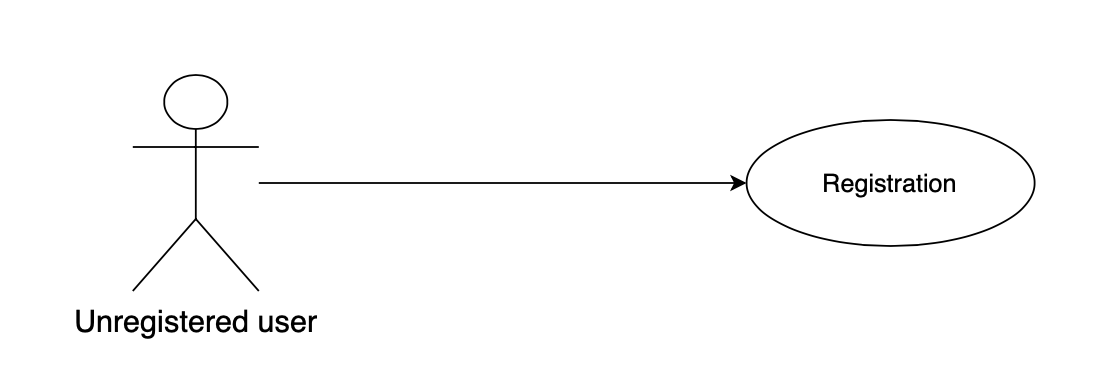
\includegraphics[scale=0.7]{images/UseCaseDiagram/UnregisteredUserUseCaseDiagram.png} 
    \caption{Unregistered user Use Case Diagram}
    \label{fig_UnregistereduserUseCaseDiagram}
\end{figure}

\clearpage
\textbf{Use Case Diagram}
\begin{figure}[h]
    \centering
    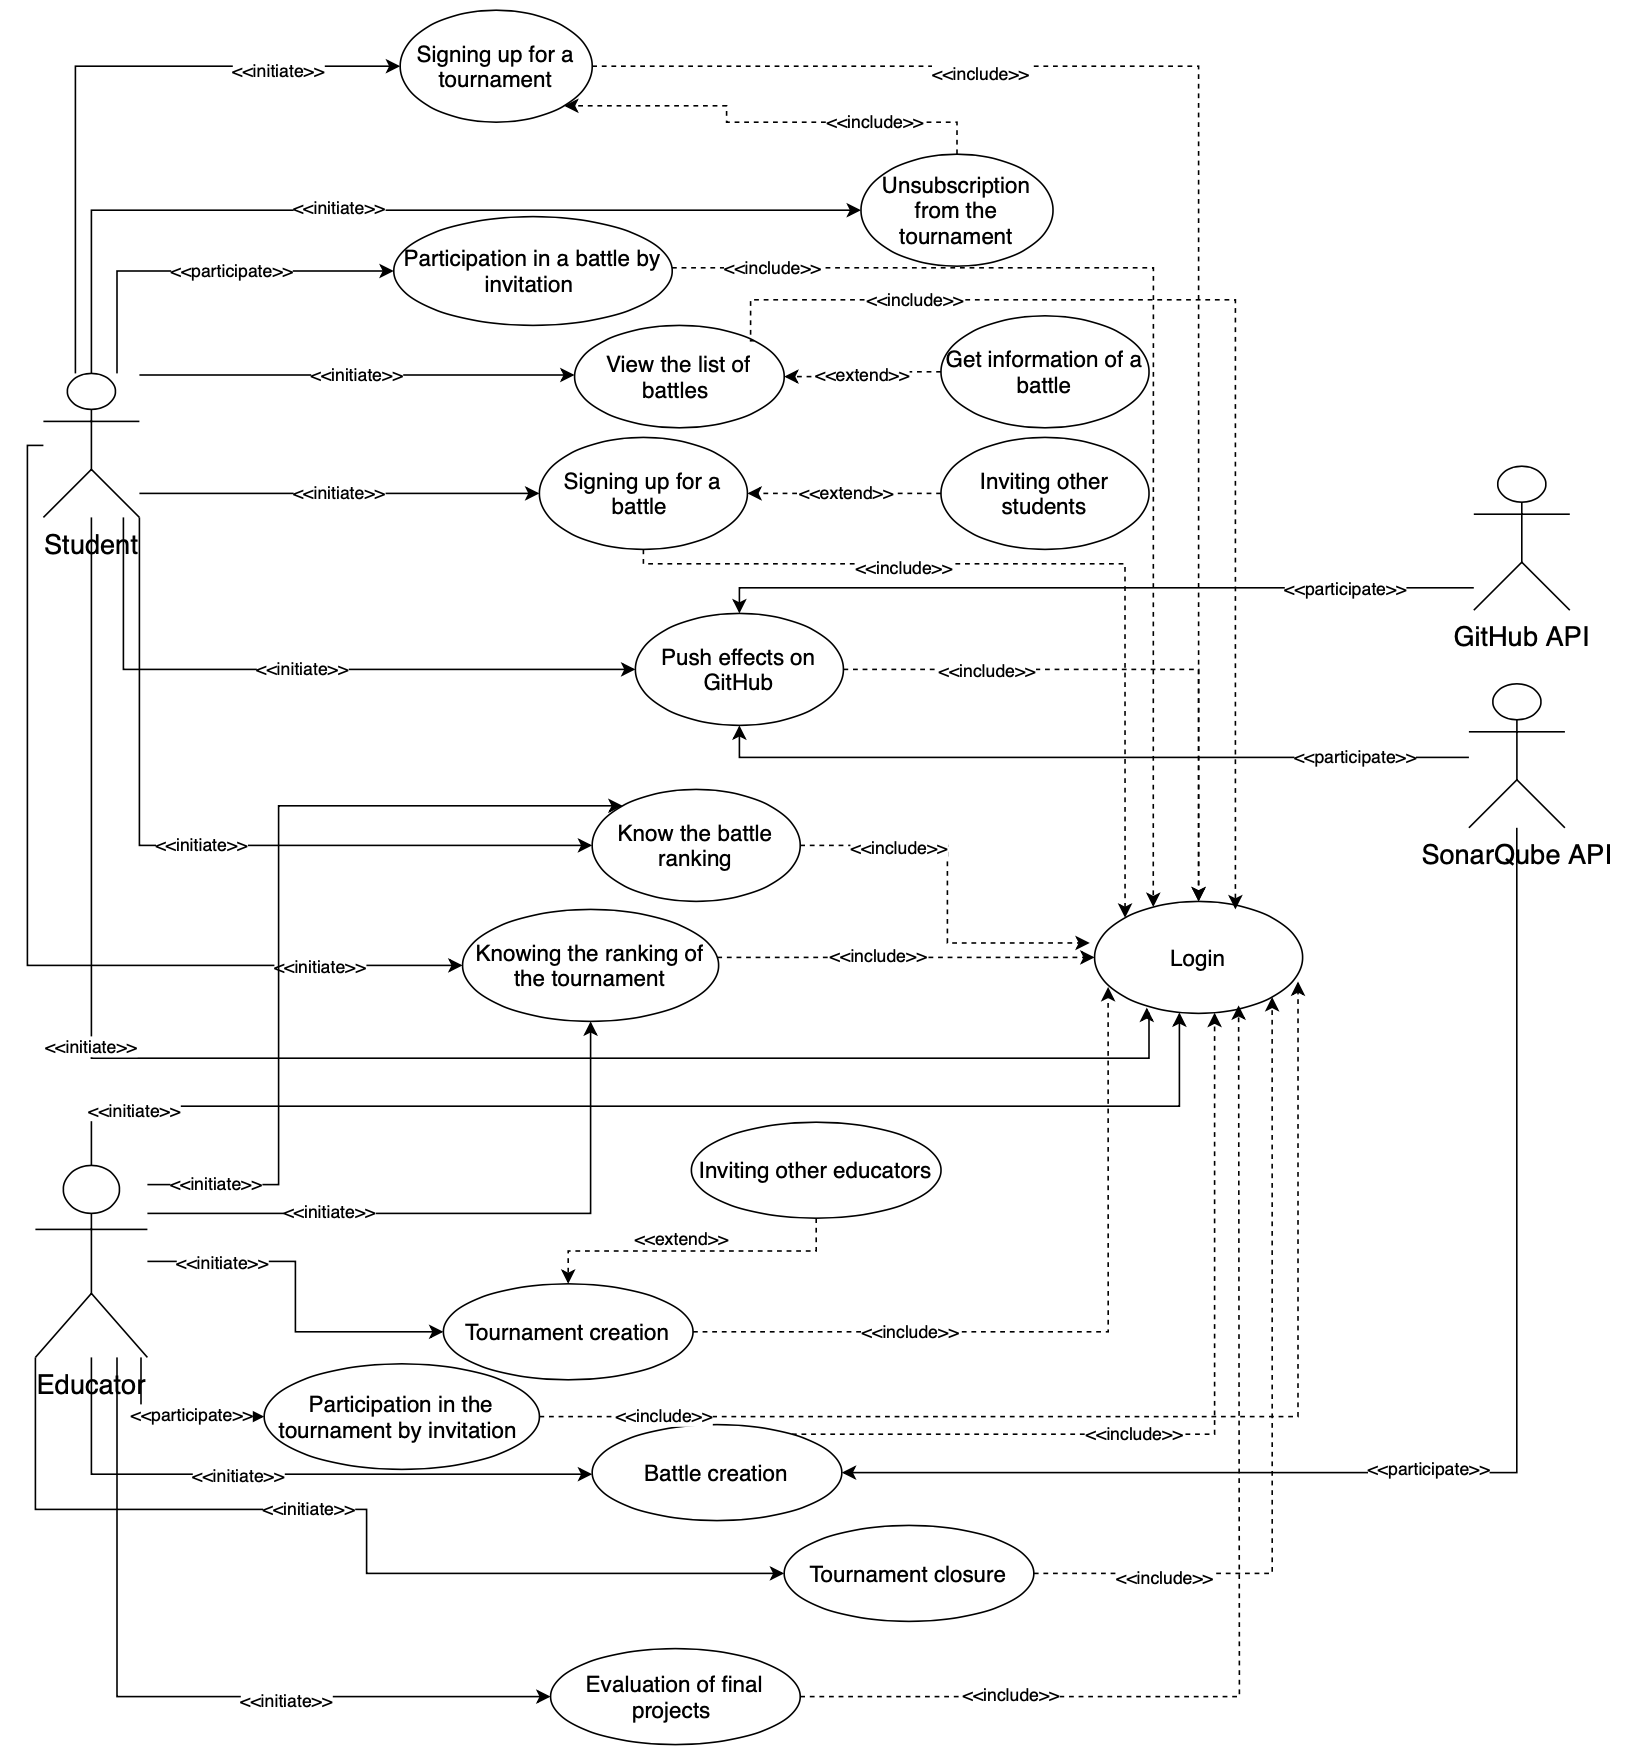
\includegraphics[scale=0.55]{images/UseCaseDiagram/UseCaseDiagram.png} 
    \caption{Use Case Diagram}
    \label{fig_StudentUseCaseDiagram}
\end{figure}


\clearpage


\subsubsection{Use Cases and Sequence Diagrams}
\vspace{1\baselineskip}
\textbf{[UC1] - Registration}

\begin{table}[h]
\begin{tabular}{|l|p{12cm}|} \hline 

\rule[-3mm]{0mm}{1cm}
\textbf{Name} & Registration \\ \hline 

\rule[-3mm]{0mm}{1cm}
\textbf{Actors} & Unregistered User \\ \hline 

\rule[-3mm]{0mm}{1cm}
\textbf{Entry Condition} & Unregistered User accesses the platform. \\ \hline 

\rule[-3mm]{0mm}{1cm}
\textbf{Event Flow} & 
\textbf{1.} Unregistered User presses on the "Sign Up" button.
\vspace{4pt}
\newline
\textbf{2.} The system shows a screen with the relevant fields:
Firstname,
Lastname,
Email,
Username,
Password.

And two buttons " Sign up as Student" and "Sign up as Educator".
\vspace{2pt}
\newline
\textbf{3.} Unregistered User fills in the fields.

\textbf{4.} Unregistered User clicks on the "Sign Up as Student" button.
\vspace{4pt}
\newline
\textbf{5.} The system displays the initial dashboard for the Student or Educator.

\\ \hline 

\rule[-3mm]{0mm}{1cm}
\textbf{Exit Condition} & Unregistered User is correctly registered as a Student or Educator. \\ \hline
\rule[-3mm]{0mm}{1cm}
\textbf{Alternative} & \textbf{4a.} Unregistered User clicks on the "Sign Up as Educator" button. \\ \hline
\end{tabular}
\end{table}

\begin{figure}[h]
    \centering
    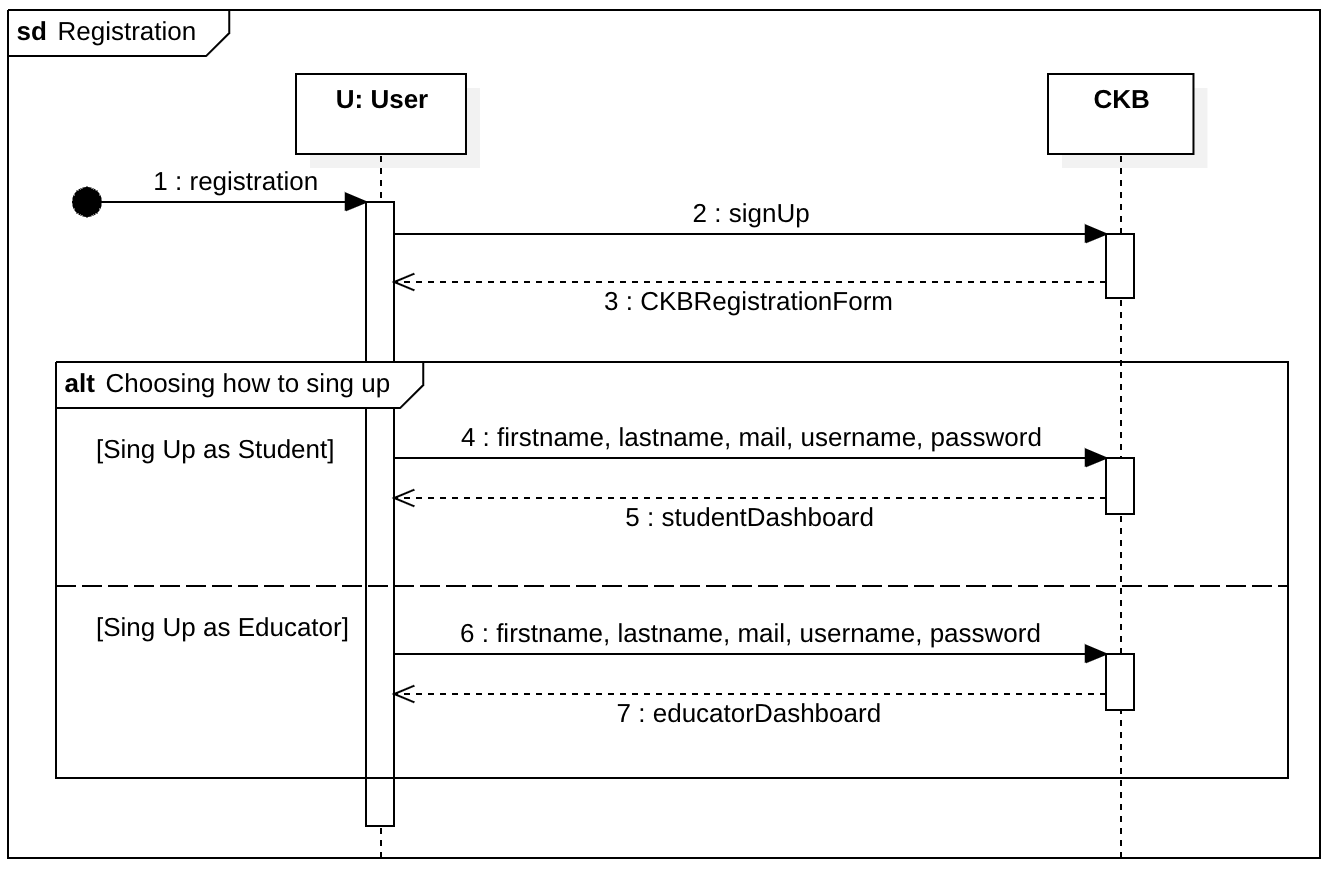
\includegraphics[scale=0.7]{images/SD/RegistrationSD.png}
    \caption{Registration Sequence Diagram}
    \label{fig_SignUpSD}
\end{figure}


\clearpage
\raggedright
\textbf{[UC2] - Login}
\begin{table}[h]
\begin{tabular}{|l|p{12cm}|} \hline 

\rule[-3mm]{0mm}{1cm}
\textbf{Name} & Login \\ \hline 

\rule[-3mm]{0mm}{1cm}
\textbf{Actors} & User  \\ \hline 

\rule[-3mm]{0mm}{1cm}
\textbf{Entry Condition} & User accesses the platform. \\ \hline 

\rule[-3mm]{0mm}{1cm}
\textbf{Event Flow} & 
\textbf{1.} User presses the "Sign In" button.
\vspace{4pt}
\newline
\textbf{2.} The system shows a screen with the relevant fields:
Username,
Password.

And two buttons " Student Login" and "Educator Login".
\vspace{2pt}
\newline
\textbf{3.} User fills in the fields.

\textbf{4a.} User clicks on the "Student Login" button.
\vspace{4pt}
\newline
\textbf{5.} The system displays the initial dashboard for the Student or Educator.

\\ \hline 

\rule[-3mm]{0mm}{1cm}
\textbf{Exit Condition} & Student or Educator are logged in correctly to the platform. \\ \hline
\rule[-3mm]{0mm}{1cm}
\textbf{Alternative} & \textbf{4b.}  User clicks on the "Educator Login" button. \\ \hline

\end{tabular}
\end{table}

\begin{figure}[h]
    \centering
    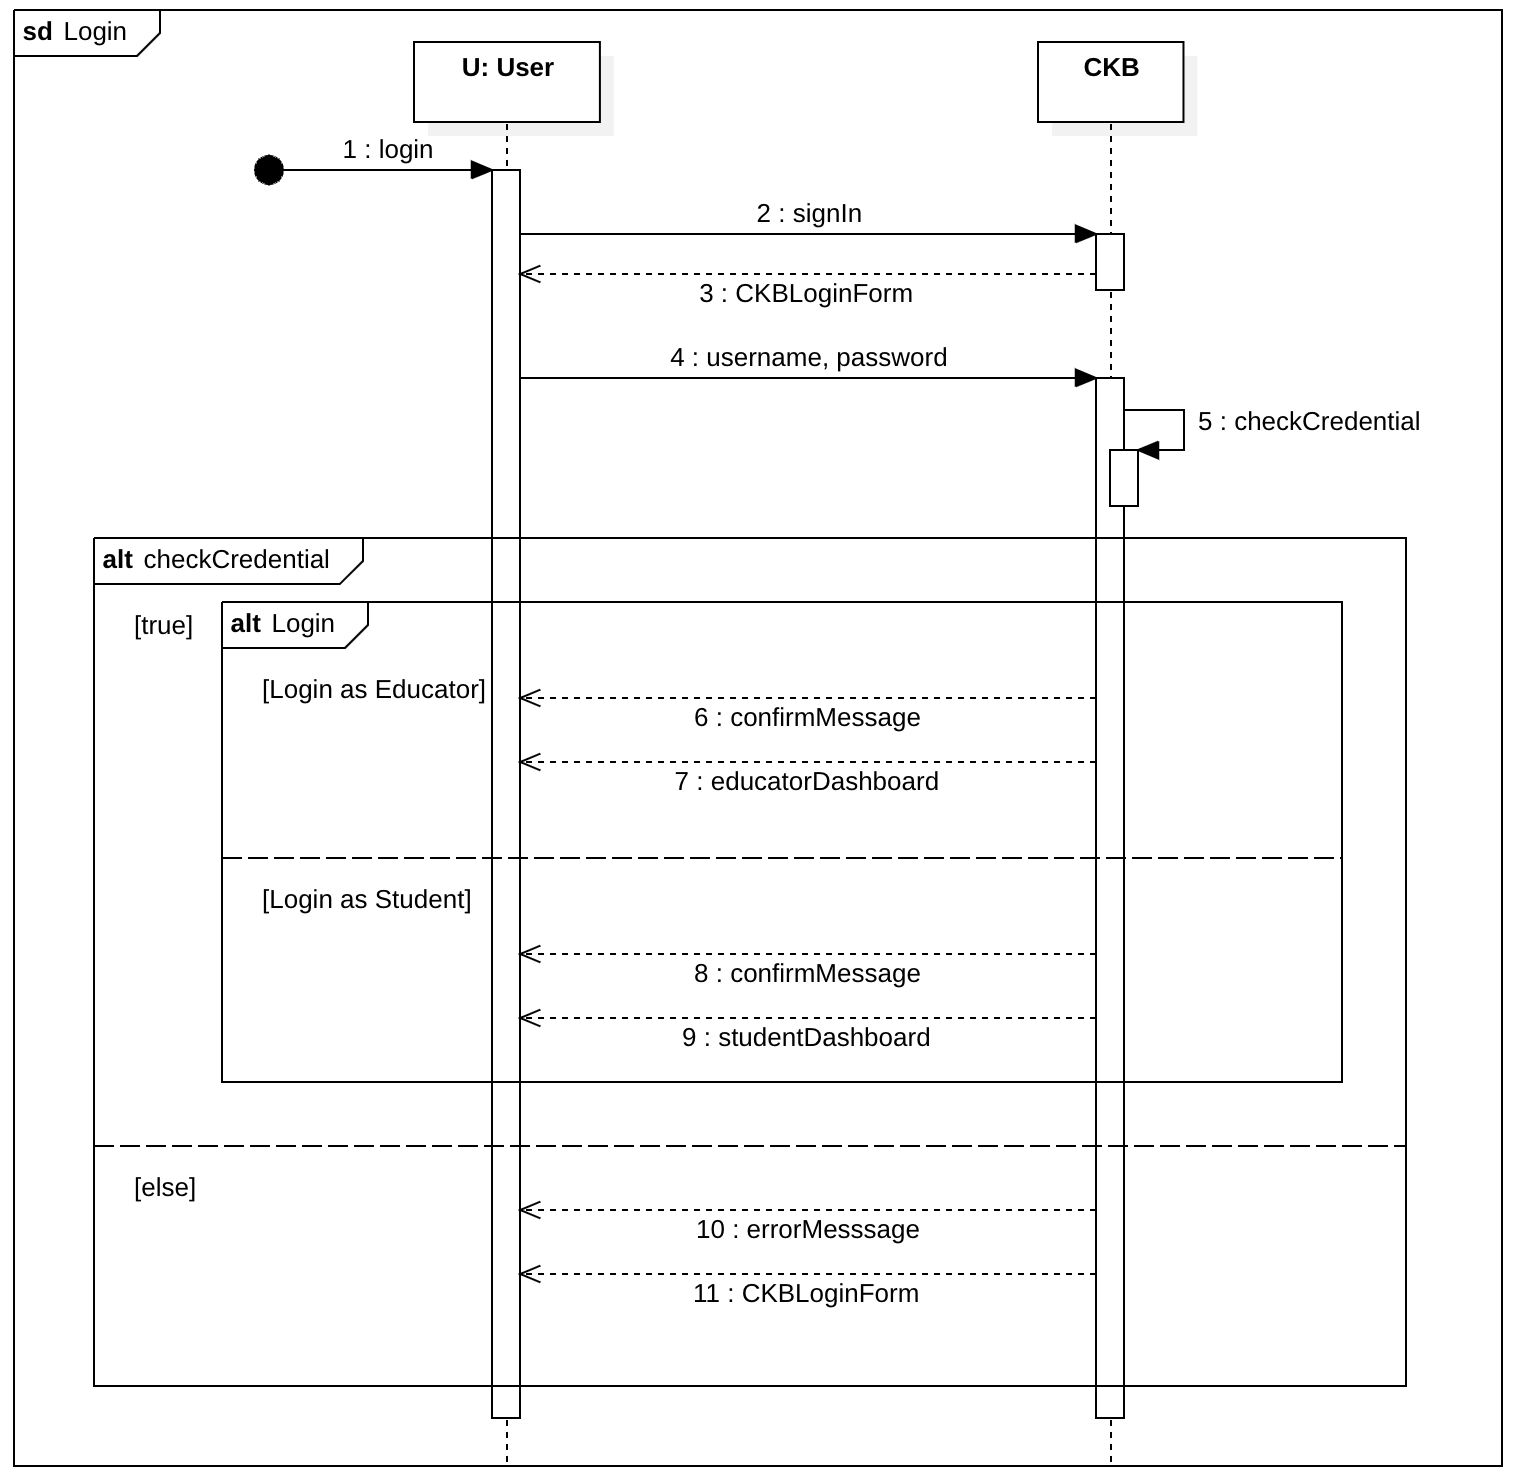
\includegraphics[scale=0.6]{images/SD/LoginSD.png}
    \caption{Sign In Sequence Diagram}
    \label{fig_SignInSD}
\end{figure}



\clearpage
\raggedright
\textbf{[UC3] - Tournament Creation}
\begin{table}[h]
\begin{tabular}{|l|p{12cm}|} \hline 

\rule[-3mm]{0mm}{1cm}
\textbf{Name} & Tournament Creation \\ \hline 

\rule[-3mm]{0mm}{1cm}
\textbf{Actors} & Educator, Student \\ \hline 

\rule[-3mm]{0mm}{1cm}
\textbf{Entry Condition} & Educator logged into the system.  \\ \hline 

\rule[-3mm]{0mm}{1cm}
\textbf{Event Flow} & 
\textbf{1.} Educator presses the "New Tournament" button.
\vspace{4pt}
\newline
\textbf{2.} The system shows him a screen with fields to fill in:
    \newline
    - Tournament name.
    \newline
    - Entry Deadline.
    \newline
    It also shows a list of educators with a checkbox next to it.
\vspace{4pt}
\newline
\textbf{3.} The educator fills in these fields and selects educators from the list.

\textbf{4.} Educator presses the "Confirm" button.
\vspace{4pt}
\newline
\textbf{5.} System notifies all students registered on the platform of the new tournament.
\vspace{4pt}
\newline
\textbf{6.} System sends a confirmation message

\\ \hline 

\rule[-3mm]{0mm}{1cm}
\textbf{Exit Condition} & The tournament was created correctly and notifications are sent correctly.  \\ \hline

\rule[-3mm]{0mm}{1cm}
\textbf{Exception} & In the event of a duplication of the tournament name, the system will ask you to enter the required fields again. \\ \hline

\end{tabular}
\end{table}

\begin{figure}[h]
    \centering
    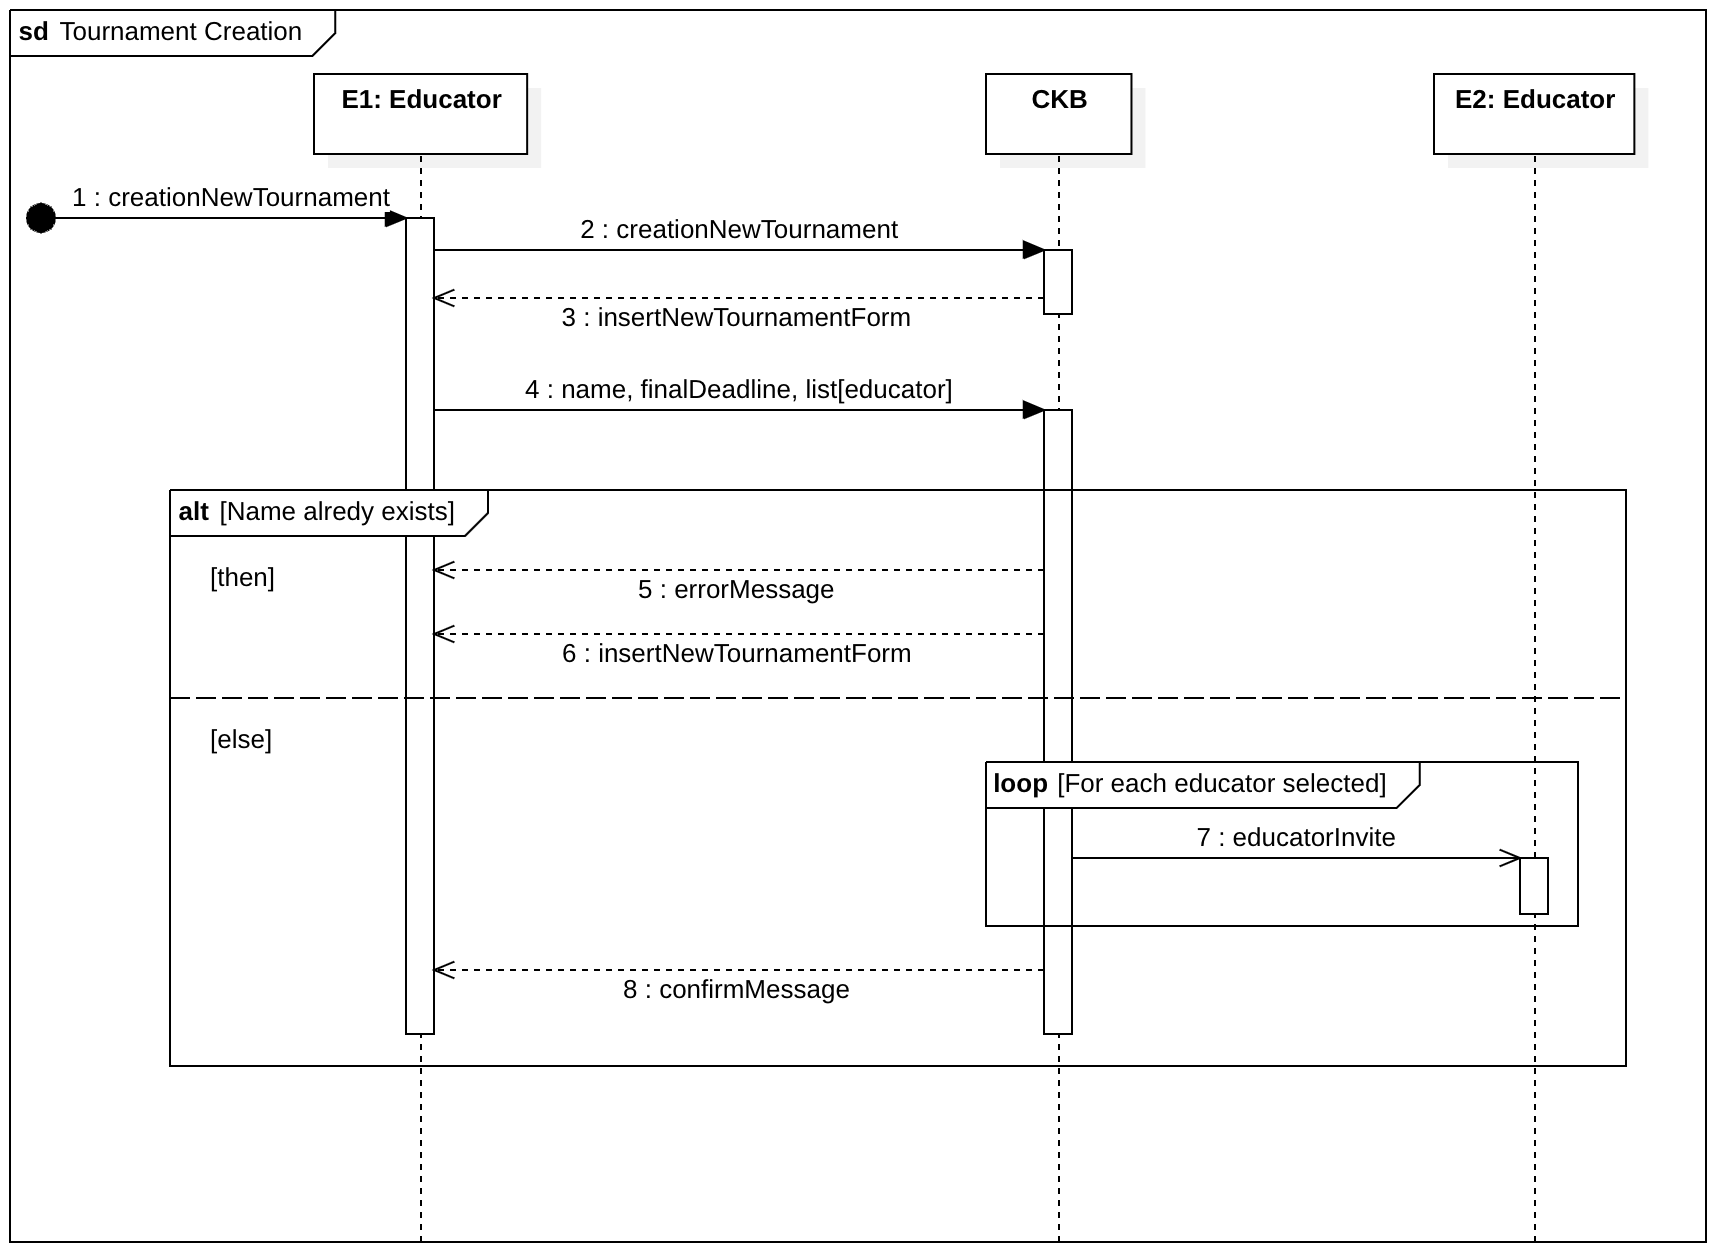
\includegraphics[scale=0.55]{images/SD/TournamentCreationSD.png}
    \caption{Tournament Creation Sequence Diagram}
    \label{fig_TournamentCreationSD}
\end{figure}



\clearpage
\raggedright
\textbf{[UC4] - Battle Creation}
\begin{table}[h]
\begin{tabular}{|l|p{12cm}|} \hline 

\rule[-3mm]{0mm}{1cm}
\textbf{Name} & Battle Creation \\ \hline 

\rule[-3mm]{0mm}{1cm}
\textbf{Actors} & Educator, SonarQube, Student \\ \hline 

\rule[-3mm]{0mm}{1cm}
\textbf{Entry Condition} & Educator logged into the system and must participate in a tournament.  
\vspace{2pt}
\\ \hline 

\rule[-3mm]{0mm}{1cm}
\textbf{Event Flow} & 
\textbf{1.} Educator presses the "Add Battle" button.
\vspace{4pt}
\newline
\textbf{2.} The system shows him a screen with fields to fill in:
    - Battle name.
    \newline
    - Registration Deadline.
    \newline
    - Minimum and maximum number of students in each group.
    \newline
    - Final project upload deadline.
    \newline
    - A field to upload the CodeKata.
    \newline
    - Aspects that must be evaluated in the source.
    \newline
    - Manual evaluation.
\vspace{4pt}
\newline
\textbf{3.} Educator fills in these fields.
\vspace{4pt}
\newline
\textbf{4.} Educator presses the "Confirm" button.
\vspace{4pt}
\newline
\textbf{5.} System sends SonaQube the aspects on which it must evaluate all the sources of each team in this battle
\vspace{4pt}
\newline
\textbf{6.} System notifies all students participating in the tournament of the new battle.
\vspace{4pt}
\newline
\textbf{7.} System sends a confirmation message

\\ \hline 

\rule[-3mm]{0mm}{1cm}
\textbf{Exit Condition} & The battle was created correctly, notifications are sent correctly and correct configuration of SonarQube. \\ \hline

\rule[-3mm]{0mm}{1cm}
\textbf{Exception} & In the event of a duplication of the battle name, the system will ask you to enter the required fields again. \\ \hline


\end{tabular}
\end{table}

\begin{figure}[h]
    \centering
    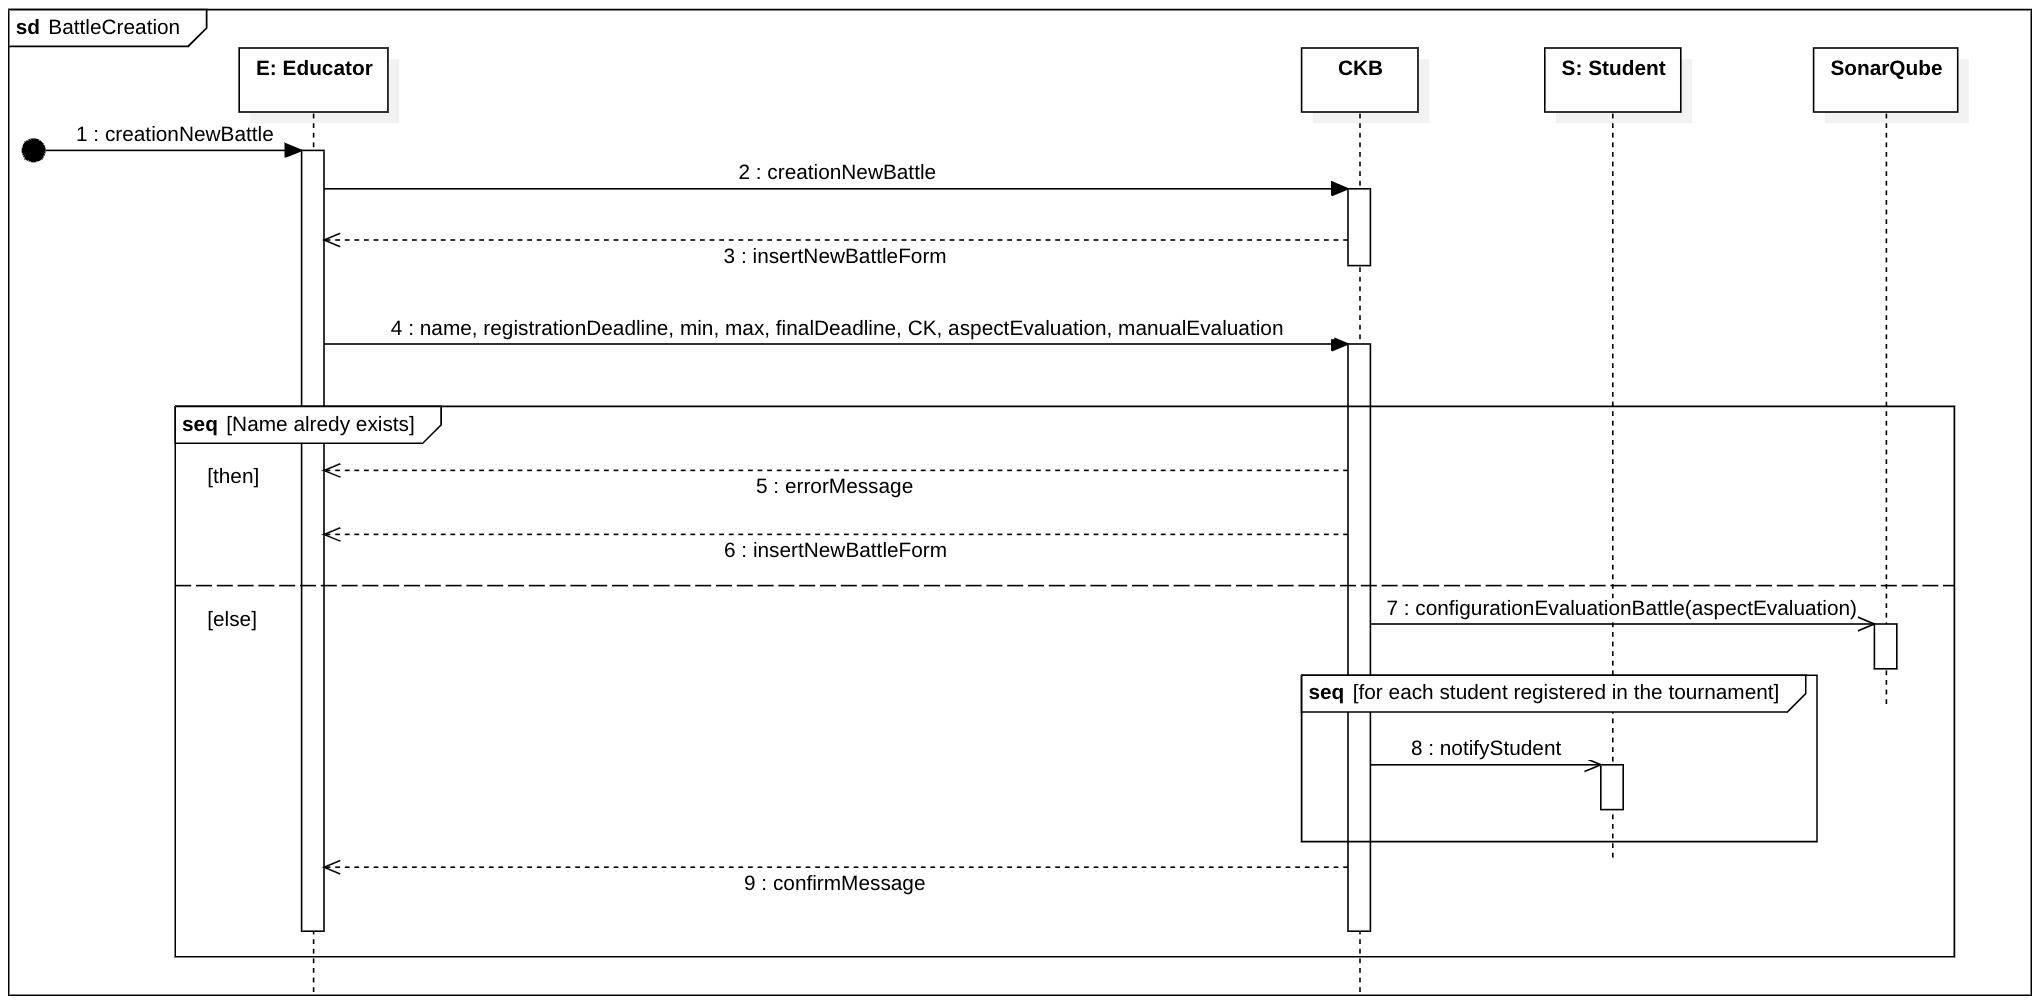
\includegraphics[scale=0.45]{images/SD/BattleCreationSD.png} 
    \caption{Battle Creation Sequence Diagram}
    \label{fig_BattleCreationSD}
\end{figure}


\clearpage
\raggedright
\textbf{[UC5] - Tournament Closing}
\begin{table}[h]
\begin{tabular}{|l|p{12cm}|} \hline 

\rule[-3mm]{0mm}{1cm}
\textbf{Name} & Tournament Closing\\ \hline 

\rule[-3mm]{0mm}{1cm}
\textbf{Actors} & Educator, Student  \\ \hline 

\rule[-3mm]{0mm}{1cm}
\textbf{Entry Condition} & Educator logged into the system, the educator who created the tournament.
\vspace{2pt}
\\ \hline 

\rule[-3mm]{0mm}{1cm}
\textbf{Event Flow} & 
\textbf{1.} Educator pushes the button on his tournament.
\vspace{4pt}
\newline
\textbf{2.} System shows him the screen of his tournament.
\vspace{4pt}
\newline
\textbf{3.} Educator presses the "Close Tournament" button.
\vspace{4pt}
\newline
\textbf{4.} System notifies all students participating in the tournament of the final ranking.
\vspace{4pt}
\newline
\textbf{5.} System sends a confirmation message

\\ \hline 

\rule[-3mm]{0mm}{1cm}
\textbf{Exit Condition} & The tournament is successfully closed and notifications are sent correctly. \\ \hline

\rule[-3mm]{0mm}{1cm}
\textbf{Exception} & The battles are not all finished. The system returns an error message. \\ \hline

\end{tabular}
\end{table}

\begin{figure}[h]
    \centering
    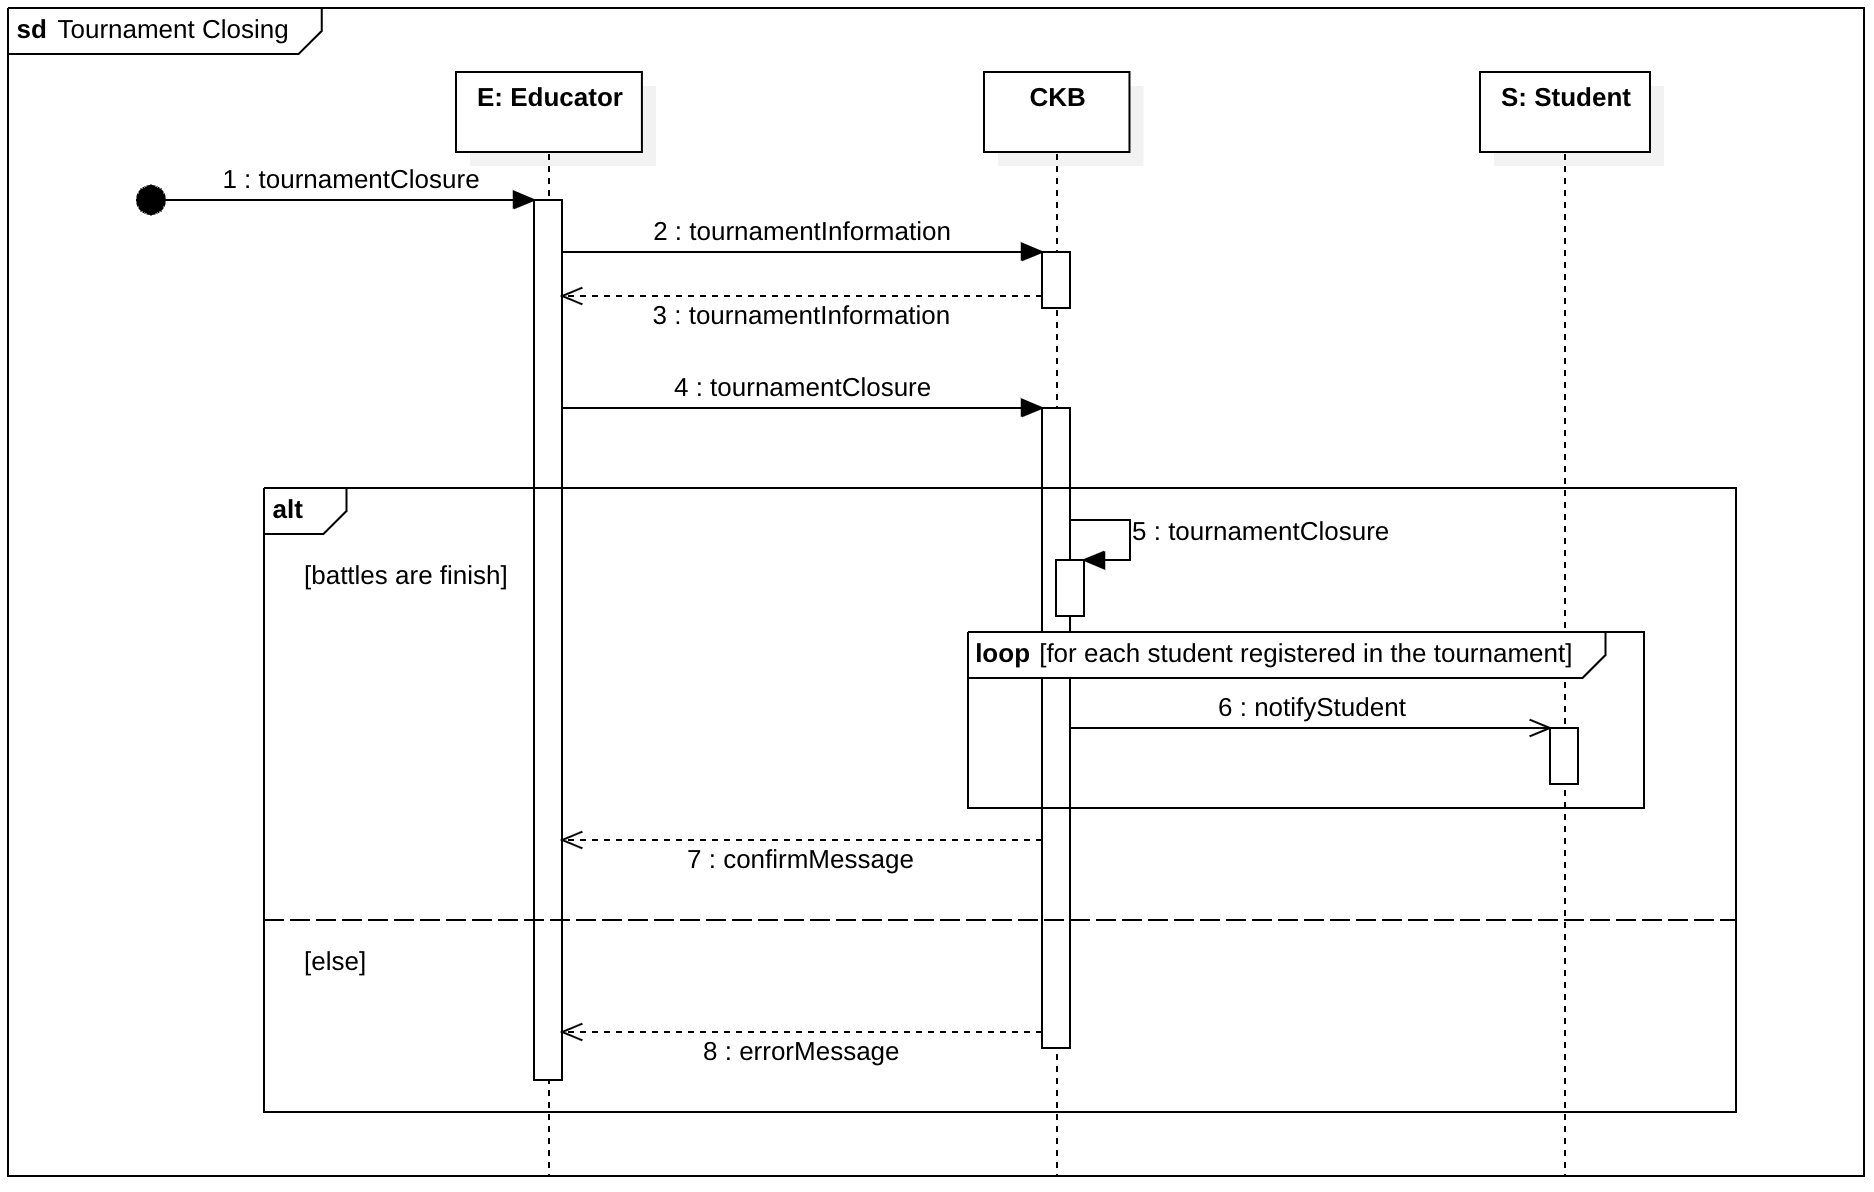
\includegraphics[scale=0.5]{images/SD/TournamentClosingSD.png} 
    \caption{Tournament Closing Sequence Diagram}
    \label{fig_TournamentClosingSD}
\end{figure}

\clearpage

\raggedright
\textbf{[UC6] - Evaluation of final project}
\begin{table}[h]
\begin{tabular}{|l|p{12cm}|} \hline 

\rule[-3mm]{0mm}{1cm}
\textbf{Name} & Evalutation of final project \\ \hline 

\rule[-3mm]{0mm}{1cm}
\textbf{Actors} & Educator \\ \hline 

\rule[-3mm]{0mm}{1cm}
\textbf{Entry Condition} & Educator connected to the system, the educator who created the battle, the battles is finished.  
\vspace{2pt}
\\ \hline 

\rule[-3mm]{0mm}{1cm}
\textbf{Event Flow} & 
\textbf{1.} Educator presses the "Final Evaluation" button.
\vspace{4pt}
\newline
\textbf{2.} System shows the screen with the list of teams inside, with a button next to it to see the latest source and a field to enter the rating.
\vspace{4pt}
\newline
\textbf{3.} The educator presses the button to examine the source of a team.
\vspace{4pt}
\newline
\textbf{5.} The system shows it the source.
\vspace{4pt}
\newline
\textbf{6.} The educator presses the button to go back.
\vspace{4pt}
\newline
\textbf{7.} System shows the previous screen.
\vspace{4pt}
\newline
\textbf{8.} Educator enters assessment to relevant team.

\\ \hline 

\rule[-3mm]{0mm}{1cm}
\textbf{Exit Condition} & Educator  assigned the assessment to each team. \\ \hline

\end{tabular}
\end{table}

\begin{figure}[h]
    \centering
    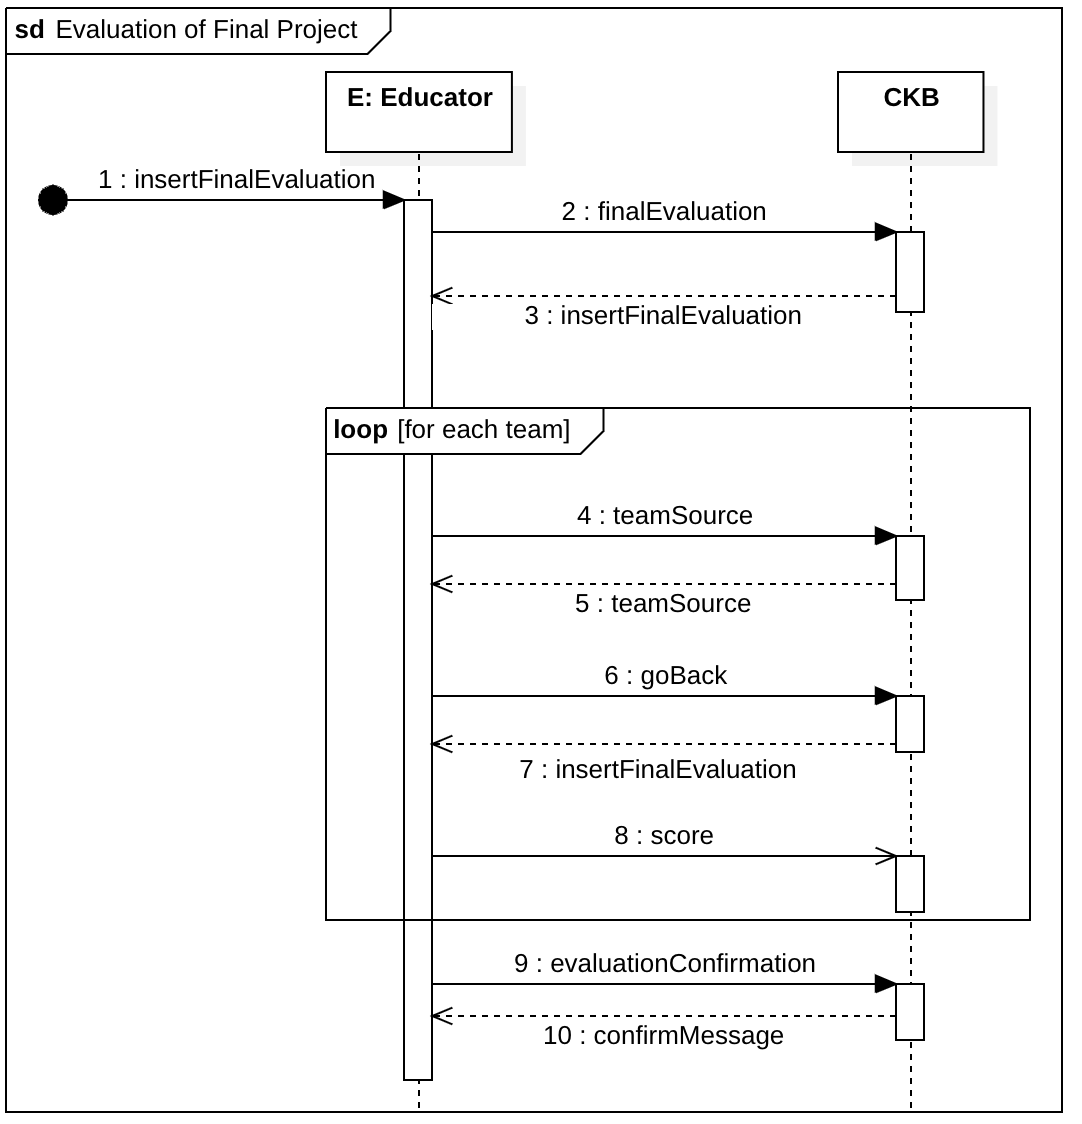
\includegraphics[scale=0.7]{images/SD/EvaluationFinalProjectSD.png} 
    \caption{Evaluation of Final Project Sequence Diagram}
    \label{fig_EvaluationFinalProjectSD}
\end{figure}

\clearpage

\raggedright
\textbf{[UC7] - Know the battle ranking}
\begin{table}[h]
\begin{tabular}{|l|p{12cm}|} \hline 

\rule[-3mm]{0mm}{1cm}
\textbf{Name} & Know the battle ranking \\ \hline 

\rule[-3mm]{0mm}{1cm}
\textbf{Actors} & Educator and Student \\ \hline 

\rule[-3mm]{0mm}{1cm}
\textbf{Entry Condition} & Actors logged into the system.
\newline
Educator created the battle.
\newline
Student is enrolled in battle.
\vspace{2pt}
\\ \hline 

\rule[-3mm]{0mm}{1cm}
\textbf{Event Flow} & 
\textbf{1.} Actors pushes the button on his battle.
\vspace{4pt}
\newline
\textbf{2.} The system shows the screen of his battle.
\vspace{4pt}
\newline
\textbf{3.} Actors presses the "Ranking" button.
\vspace{4pt}
\newline
\textbf{4.} System shows screen with battle ranking.

\\ \hline 

\rule[-3mm]{0mm}{1cm}
\textbf{Exit Condition} & Actors sees ranking of teams. \\ \hline

\end{tabular}
\end{table}

\begin{figure}[h]
    \centering
    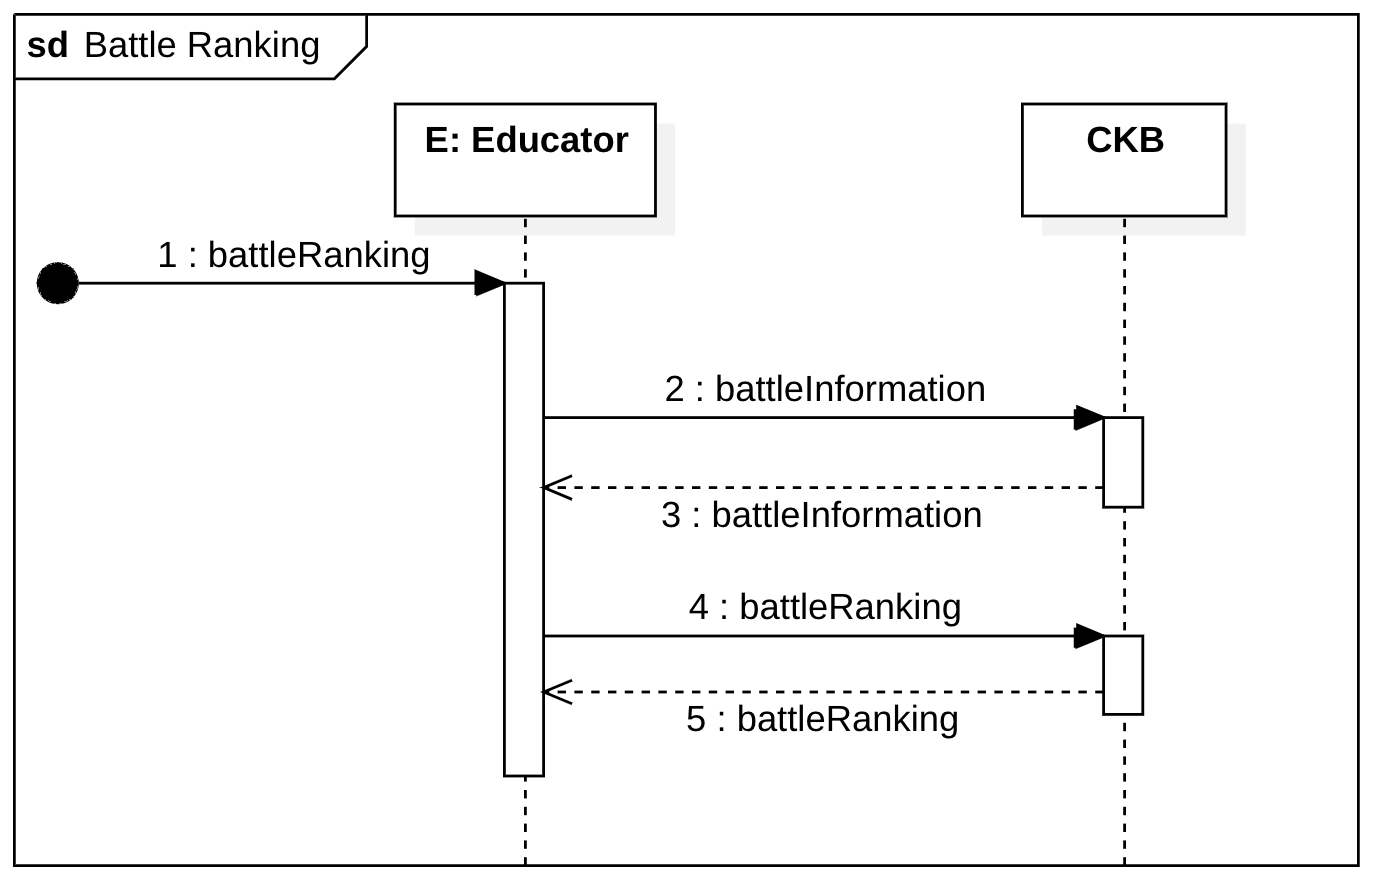
\includegraphics[scale=0.5]{images/SD/RankingBattleSD.png} 
    \caption{Battle Ranking Sequence Diagram, same for student}
    \label{fig_RankingBattleSD}
\end{figure}

\clearpage

\raggedright
\textbf{[UC8] - Know the tournament ranking}
\begin{table}[h]
\begin{tabular}{|l|p{12cm}|} \hline 

\rule[-3mm]{0mm}{1cm}
\textbf{Name} & Know the tournament ranking \\ \hline 

\rule[-3mm]{0mm}{1cm}
\textbf{Actors} & Registered Users  \\ \hline 

\rule[-3mm]{0mm}{1cm}
\textbf{Entry Condition} & User logged into the system.
\vspace{2pt}
\\ \hline 

\rule[-3mm]{0mm}{1cm}
\textbf{Event Flow} & 
\textbf{1.} User select tournament to view.
\vspace{4pt}
\newline
\textbf{2.} System shows them the tournament page.
\vspace{4pt}
\newline
\textbf{3.} User press on the "Score Ranking" button.
\vspace{4pt}
\newline
\textbf{4.} The system displays a page with the ranking and score of each student entered in the tournament.

\\ \hline 

\rule[-3mm]{0mm}{1cm}
\textbf{Exit Condition} & User take a look at the ranking. \\ \hline

\end{tabular}
\end{table}

\begin{figure}[h]
    \centering
    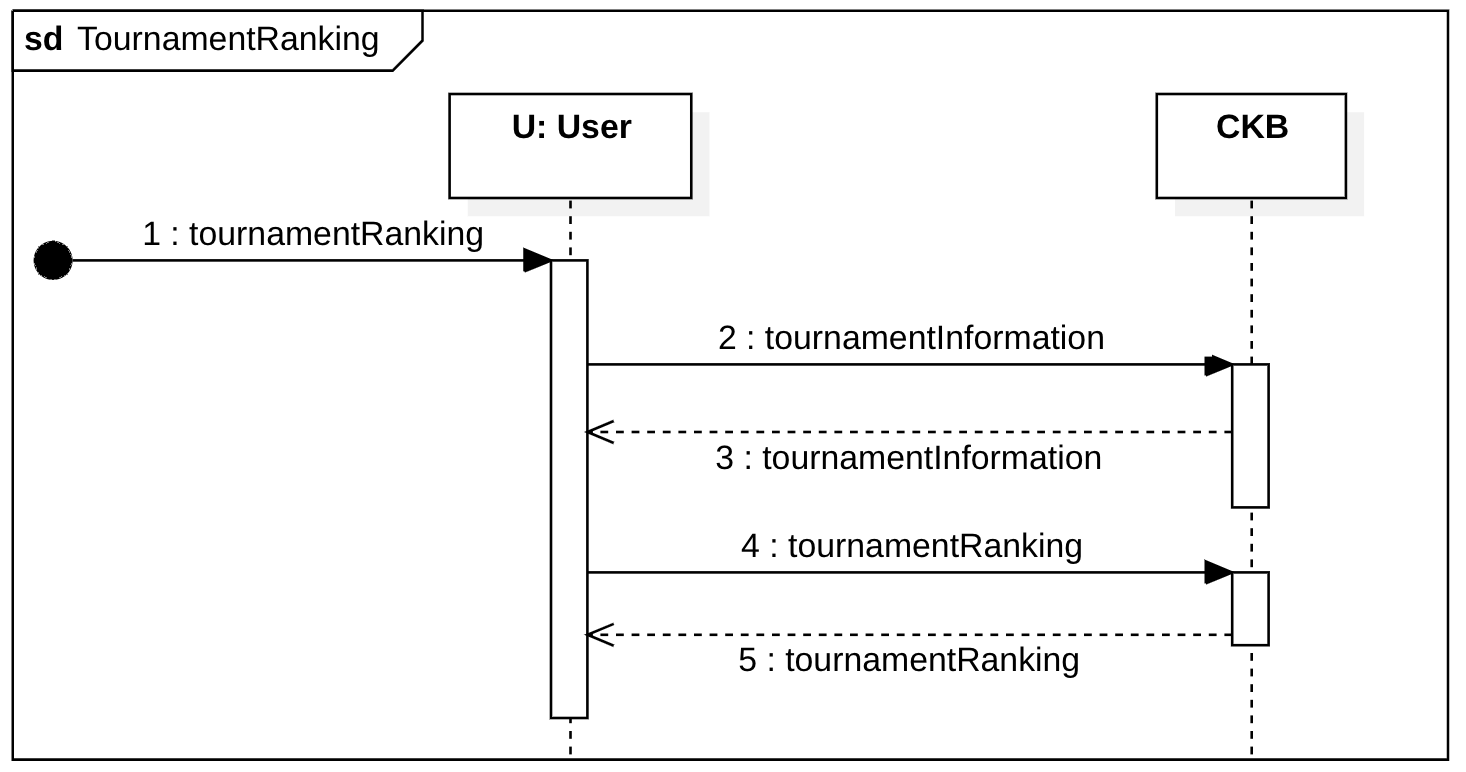
\includegraphics[scale=0.6]{images/SD/TournamentRankingSD.png} 
    \caption{Tournament Ranking Sequence Diagram}
    \label{fig_RankingTournamentSD}
\end{figure}

\clearpage

\raggedright
\textbf{[UC9] - Signing up for a tournament}
\begin{table}[h]
\begin{tabular}{|l|p{12cm}|} \hline 

\rule[-3mm]{0mm}{1cm}
\textbf{Name} & Signing up for a tournament \\ \hline 

\rule[-3mm]{0mm}{1cm}
\textbf{Actors} & Student \\ \hline 

\rule[-3mm]{0mm}{1cm}
\textbf{Entry Condition} & Student logged into the system.
\vspace{2pt}
\\ \hline 

\rule[-3mm]{0mm}{1cm}
\textbf{Event Flow} & 
\textbf{1.} Student accesses the system.
\vspace{4pt}
\newline
\textbf{2.} System shows screen with available tournaments.
\vspace{4pt}
\newline
\textbf{3.} Student presses on a tournament.
\vspace{4pt}
\newline
\textbf{4.} System shows the tournament screen, with related information such as creator and registration deadline.
\vspace{4pt}
\newline
\textbf{5.} Student presses the "Enrollment" button.
\vspace{4pt}
\newline
\textbf{6.} System sends a confirmation message.

\\ \hline 

\rule[-3mm]{0mm}{1cm}
\textbf{Exit Condition} & Student successfully enrolled in tournament. \\ \hline

\end{tabular}
\end{table}

\begin{figure}[h]
    \centering
    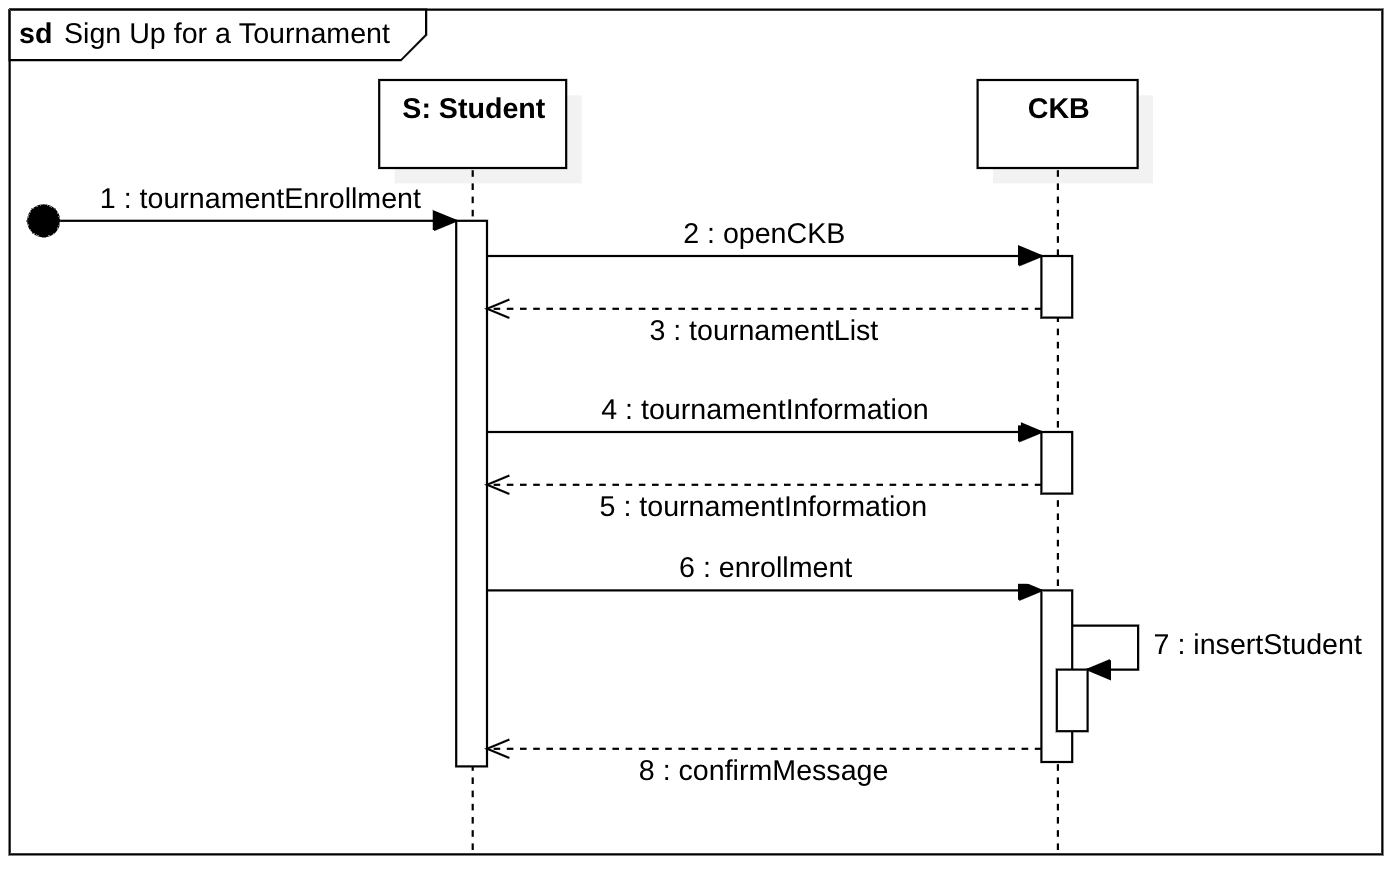
\includegraphics[scale=0.6]{images/SD/SignUpTournamentSD.png} 
    \caption{Sign Up for a Tournament Sequence Diagram}
    \label{fig_SignUpTournamentSD}
\end{figure}

\clearpage

\raggedright
\textbf{[UC10] - Unsubscription from the tournament}
\begin{table}[h]
\begin{tabular}{|l|p{12cm}|} \hline 

\rule[-3mm]{0mm}{1cm}
\textbf{Name} & Unsubscription from the tournament \\ \hline 

\rule[-3mm]{0mm}{1cm}
\textbf{Actors} & Student \\ \hline 

\rule[-3mm]{0mm}{1cm}
\textbf{Entry Condition} & Student logged into the system and student is enrolled in a tournament.
\vspace{2pt}
\\ \hline 

\rule[-3mm]{0mm}{1cm}
\textbf{Event Flow} & 
\textbf{1.} Student presses the tournament button where he participates.
\vspace{4pt}
\newline
\textbf{2.} The system shows the tournament screen.
\vspace{4pt}
\newline
\textbf{3.} Student presses on "unsubscribe" button.
\vspace{4pt}
\newline
\textbf{4.} System removes student from tournament participants and ranking and sends a confirmation message.

\\ \hline 

\rule[-3mm]{0mm}{1cm}
\textbf{Exit Condition} & Student unsubscribe correctly. \\ \hline

\end{tabular}
\end{table}

\begin{figure}[h]
    \centering
    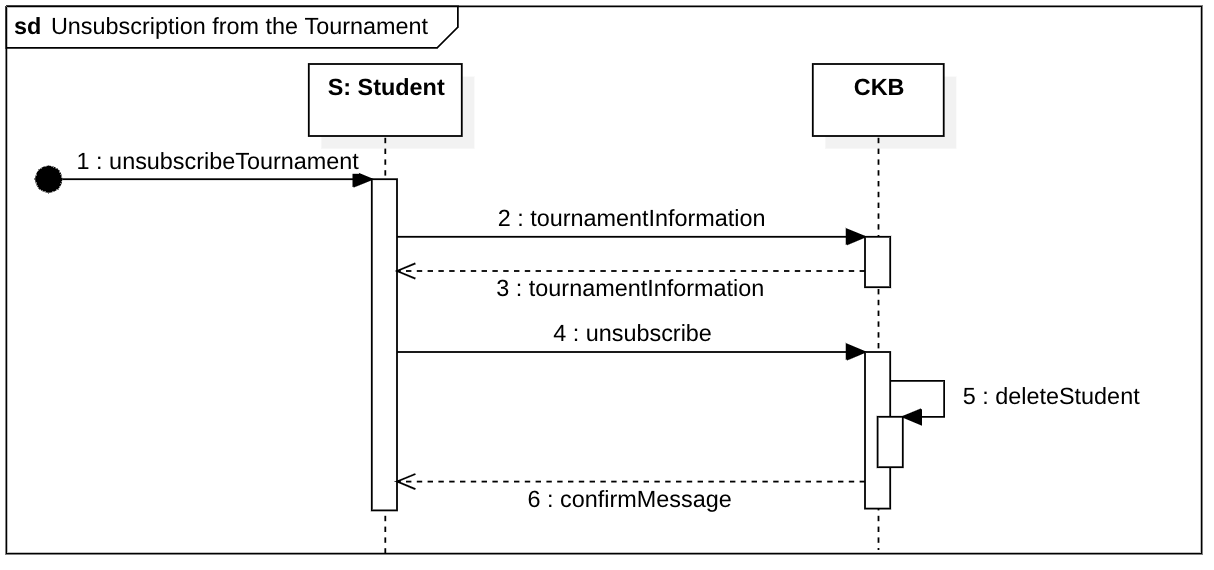
\includegraphics[scale=0.77]{images/SD/UnsubscriptionTournamentSD.png} 
    \caption{Unsubscription from the Tournament Sequence Diagram}
    \label{fig_UnsubscriptionTournamentSD}
\end{figure}

\clearpage
\raggedright
\textbf{[UC11] - View the list of battles}
\begin{table}[h]
\begin{tabular}{|l|p{12cm}|} \hline 

\rule[-3mm]{0mm}{1cm}
\textbf{Name} & View the list of battles \\ \hline 

\rule[-3mm]{0mm}{1cm}
\textbf{Actors} & Student \\ \hline 

\rule[-3mm]{0mm}{1cm}
\textbf{Entry Condition} & Student logged into the system and registered for a tournament.
\vspace{2pt}
\\ \hline 

\rule[-3mm]{0mm}{1cm}
\textbf{Event Flow} & 
\textbf{1.} Student presses on his tournament button.
\vspace{4pt}
\newline
\textbf{2.} System shows the tournament screen, with all the battles.
\vspace{4pt}
\newline
\textbf{3.} Student presses on a battle.
\vspace{4pt}
\newline
\textbf{4.} The system shows the screen with all the information related to that battle.

\\ \hline 

\rule[-3mm]{0mm}{1cm}
\textbf{Exit Condition} & Student reviews the battles. \\ \hline

\end{tabular}
\end{table}

\begin{figure}[h]
    \centering
    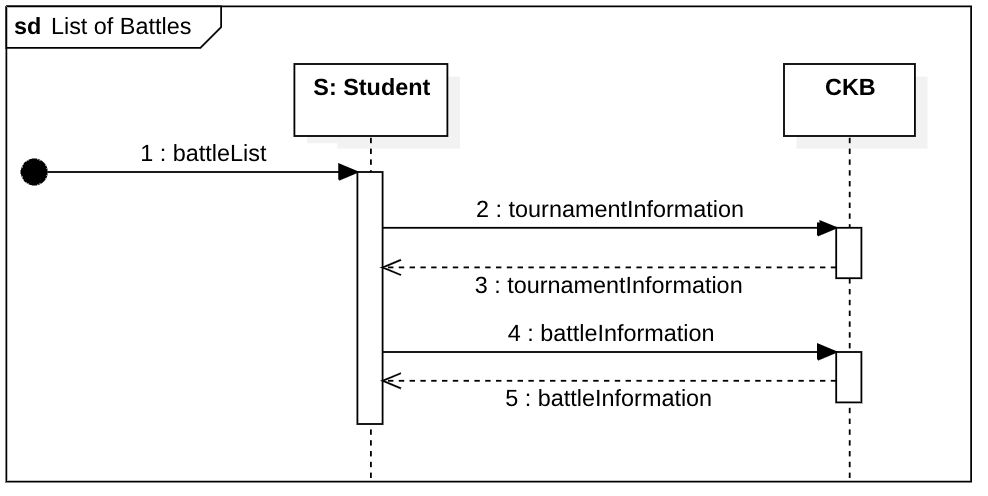
\includegraphics[scale=0.9]{images/SD/ListBattleSD.png} 
    \caption{View the list of battles Sequence Diagram}
    \label{fig_ListBattletSD}
\end{figure}



\clearpage
\raggedright
\textbf{[UC12] - Signing up for a battle}
\begin{table}[h]
\begin{tabular}{|l|p{12cm}|} \hline 

\rule[-3mm]{0mm}{1cm}
\textbf{Name} & Signing up for a battle \\ \hline 

\rule[-3mm]{0mm}{1cm}
\textbf{Actors} & Student \\ \hline 

\rule[-3mm]{0mm}{1cm}
\textbf{Entry Condition} & Student logged into the system and registered for a tournament.
\vspace{2pt}
\\ \hline 

\rule[-3mm]{0mm}{1cm}
\textbf{Event Flow} & 
\textbf{1.} Student selects the battle that has not yet begun.
\vspace{4pt}
\newline
\textbf{2.} The system displays the battle page with inside: 
the relevant information, a field to enter the team name, a list of students with a check box next to it, and the "Join" button.
\vspace{4pt}
\newline
\textbf{3.} The student fills in the text field and selects the students they wish to invite using a checkbox.
\vspace{4pt}
\newline
\textbf{4.} Student presses the "Join" button.
\vspace{4pt}
\newline
\textbf{5.} System notifies all students selected by the student to participate in his team.
\vspace{4pt}
\newline
\textbf{6.} The system displays a confirmation message.

\vspace{4pt}

\\ \hline 

\rule[-3mm]{0mm}{1cm}
\textbf{Exit Condition} & The student is ready to work on the project. \\ \hline

\end{tabular}
\end{table}

\clearpage
\begin{figure}[h]
    \centering
    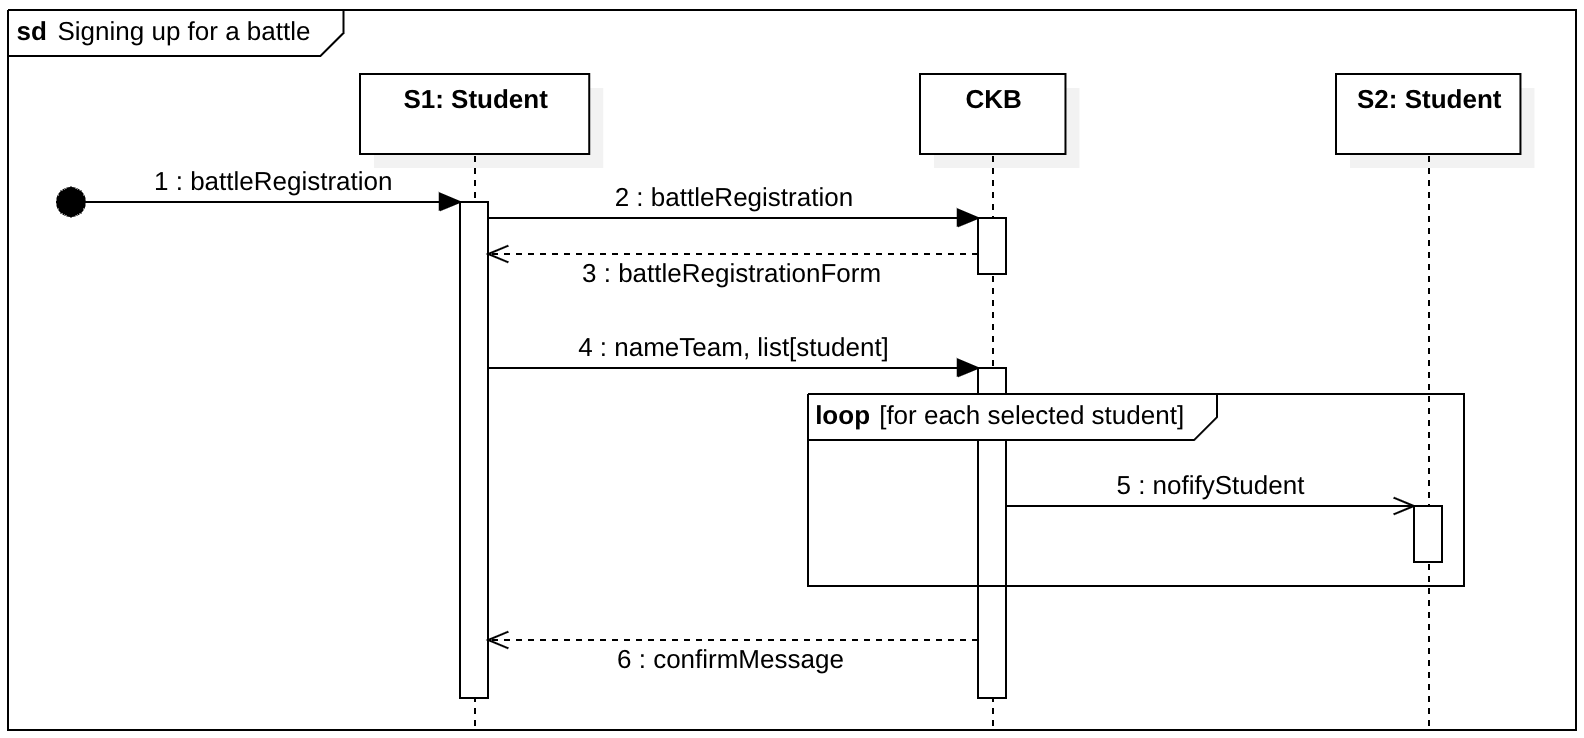
\includegraphics[scale=0.6]{images/SD/SigningUpBattleSD.png} 
    \caption{Signing up for a battle Sequence Diagram}
    \label{fig_SigningUpBattleSD}
\end{figure}

\clearpage
\raggedright
\textbf{[UC13] - Push effects on GitHub}
\begin{table}[h]
\begin{tabular}{|l|p{12cm}|} \hline 

\rule[-3mm]{0mm}{1cm}
\textbf{Name} & Push effects on GitHub \\ \hline 

\rule[-3mm]{0mm}{1cm}
\textbf{Actors} & Student, GitHub and SonarQube \\ \hline 

\rule[-3mm]{0mm}{1cm}
\textbf{Entry Condition} & Student logged into the system and registered to a battle.
\vspace{2pt}
\\ \hline 

\rule[-3mm]{0mm}{1cm}
\textbf{Event Flow} & 
\textbf{1.} Student makes a push on his GitHub repository of the new source.
\vspace{4pt}
\newline
\textbf{2.} System is informed by GitHub that the team in which the student participates has made a new push to GitHub.
\vspace{4pt}
\newline
\textbf{3.} System pulls on the student team's GitHub repository. 
\vspace{4pt}
\newline
\textbf{4.} System sends the retrieved source code to SonarQube to perform static analysis of the code and be evaluated on the aspects entered by the educator at the battle creation stage.
\vspace{4pt}
\newline
\textbf{5.} System once received the data from SonarQube completes the evaluation, also calculating timeliness and functional aspects, scoring the project from 0 to 100.
\vspace{4pt}
\newline
\textbf{6.} System updates the team's current score with the new score and updates the ranking.

\\\hline 

\rule[-3mm]{0mm}{1cm}
\textbf{Exit Condition} & Student's team score and battle ranking is updated correctly.  \\ \hline

\end{tabular}
\end{table}

\begin{figure}[h]
    \centering
    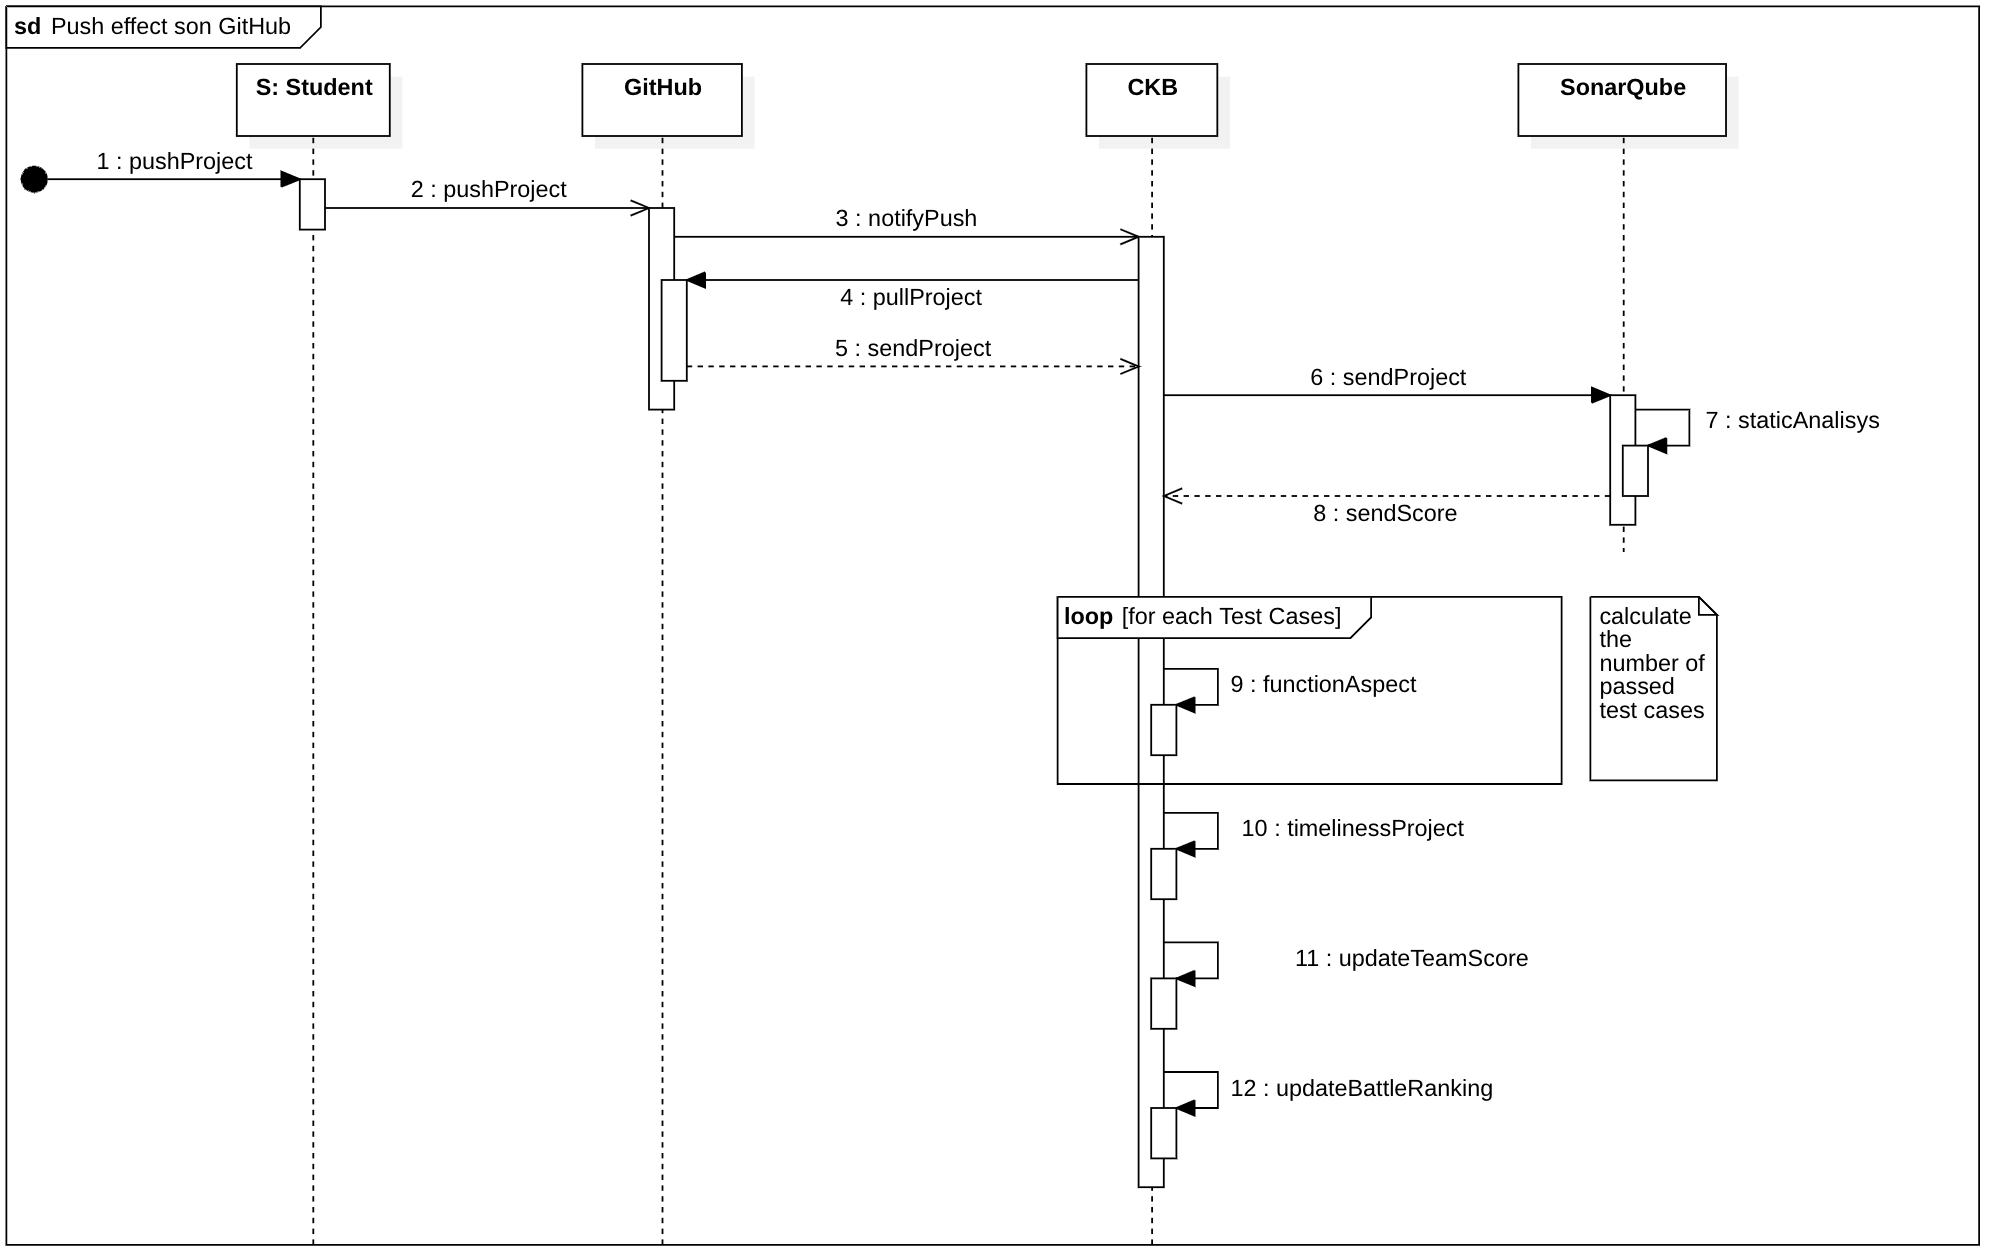
\includegraphics[scale=0.5]{images/SD/PushGitHubSD.png} 
    \caption{Push effects on GitHub Sequence Diagram}
    \label{fig_PushGitHubSD}
\end{figure}


\clearpage
\raggedright
\textbf{[UC14] - Participation in a battle by invitation}
\begin{table}[h]
\begin{tabular}{|l|p{12cm}|} \hline 

\rule[-3mm]{0mm}{1cm}
\textbf{Name} &  Participation in a battle by invitation \\ \hline 

\rule[-3mm]{0mm}{1cm}
\textbf{Actors} & Student \\ \hline 

\rule[-3mm]{0mm}{1cm}
\textbf{Entry Condition} & Student logged into the system and registered for a tournament
\vspace{2pt}
\\ \hline 

\rule[-3mm]{0mm}{1cm}
\textbf{Event Flow} & 
\textbf{1.} The system sends a notification to the Student requesting to join a team.
\vspace{4pt}
\newline
\textbf{2.} The Student requests notifications.
\vspace{4pt}
\newline
\textbf{3.} The System displays the notifications.
\vspace{4pt}
\newline
\textbf{4a.} The Student accepts the invitation.
\vspace{4pt}
\newline
\textbf{5.} System sends a confirmation message. 

\\\hline 


\rule[-3mm]{0mm}{1cm}
\textbf{Exit Condition} & The Student is a member of the team. \\ \hline

\rule[-3mm]{0mm}{1cm}
\textbf{Alternative} & \textbf{4b.} The Student declines the invitation. \\ \hline

\rule[-3mm]{0mm}{1cm}
\textbf{Exception} & The battle has already begun. The system sends an error message. \\ \hline

\end{tabular}
\end{table}

\clearpage
\begin{figure}[h]
    \centering
    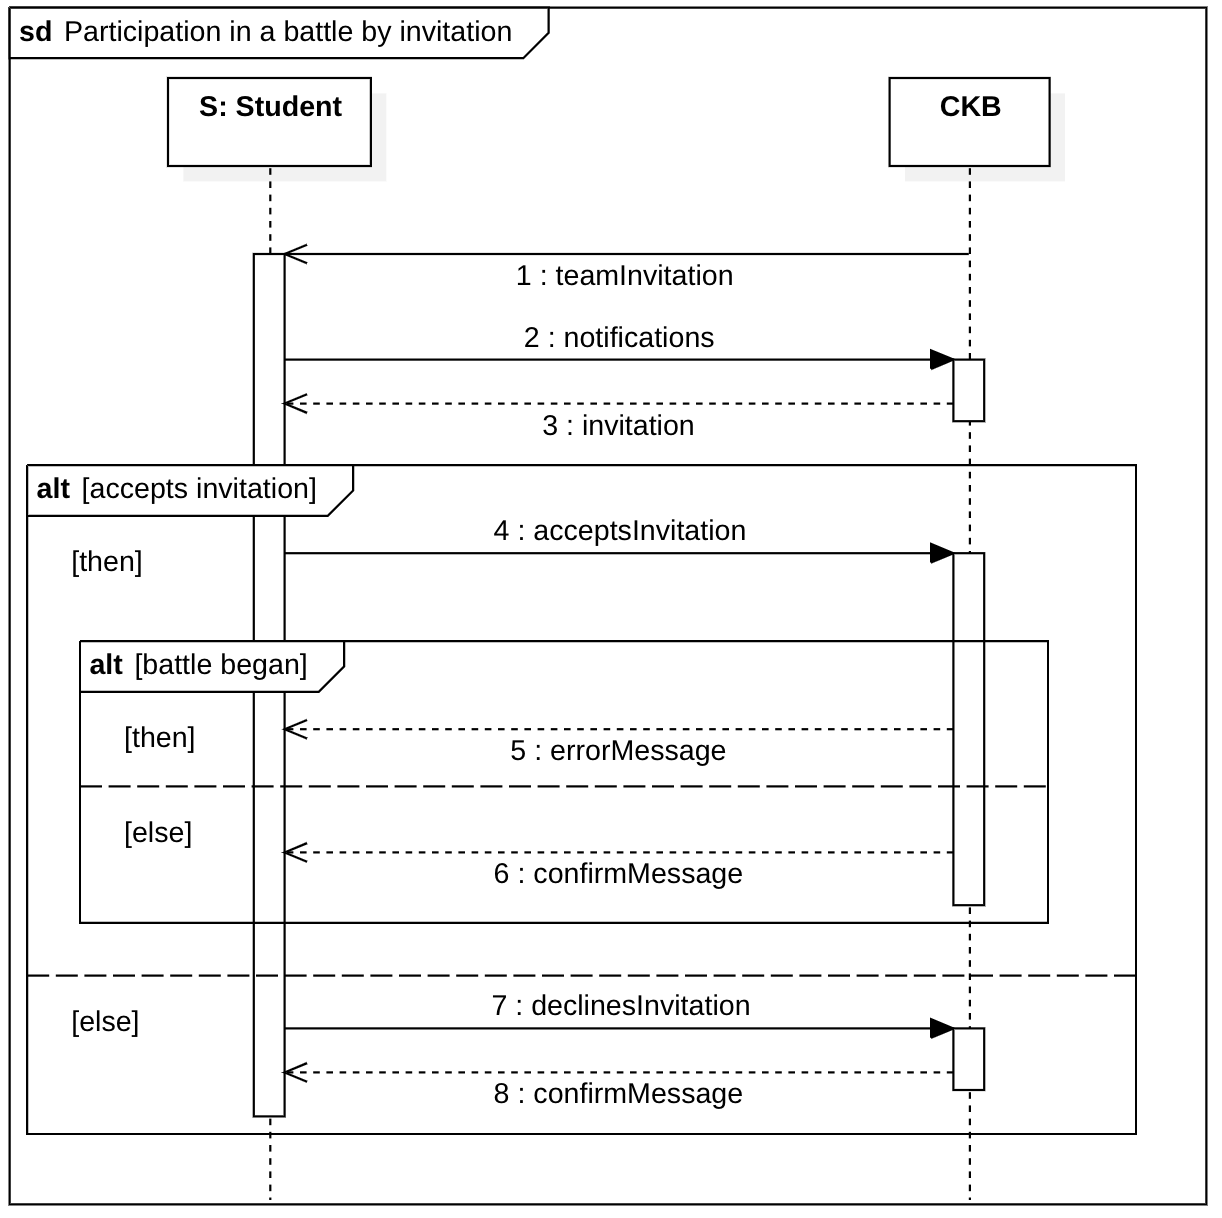
\includegraphics[scale=0.6]{images/SD/ParticipationBattleInvitationSD.png} 
    \caption{Participation in a Battle by invitation Sequence Diagram}
    \label{fig_SignUpTournamentSD}
\end{figure}

%\clearpage


\clearpage
\raggedright
\textbf{[UC15] - Participation in a tournament by invitation}
\begin{table}[h]
\begin{tabular}{|l|p{12cm}|} \hline 

\rule[-3mm]{0mm}{1cm}
\textbf{Name} &  Participation in a tournament by invitation \\ \hline 

\rule[-3mm]{0mm}{1cm}
\textbf{Actors} & Educator \\ \hline 

\rule[-3mm]{0mm}{1cm}
\textbf{Entry Condition} & Educator logged into the system.
\vspace{2pt}
\\ \hline 

\rule[-3mm]{0mm}{1cm}
\textbf{Event Flow} & 
\textbf{1.} The system sends a notification to the Educator asking to join a tournament.
\vspace{4pt}
\newline
\textbf{2.} The Educator requests notifications.
\vspace{4pt}
\newline
\textbf{3.} The System displays the notifications.
\vspace{4pt}
\newline
\textbf{4a.} The Educator accepts the invitation.
\vspace{4pt}
\newline
\textbf{5.} System sends a confirmation message. 

\\\hline 


\rule[-3mm]{0mm}{1cm}
\textbf{Exit Condition} & The Educator is a member of the tournament. \\ \hline

\rule[-3mm]{0mm}{1cm}
\textbf{Alternative} & \textbf{4b.} The Educator declines the invitation. \\ \hline

\rule[-3mm]{0mm}{1cm}
\textbf{Exception} & The tournament has already begun. The system sends an error message. \\ \hline

\end{tabular}
\end{table}

\clearpage
\begin{figure}[h]
    \centering
    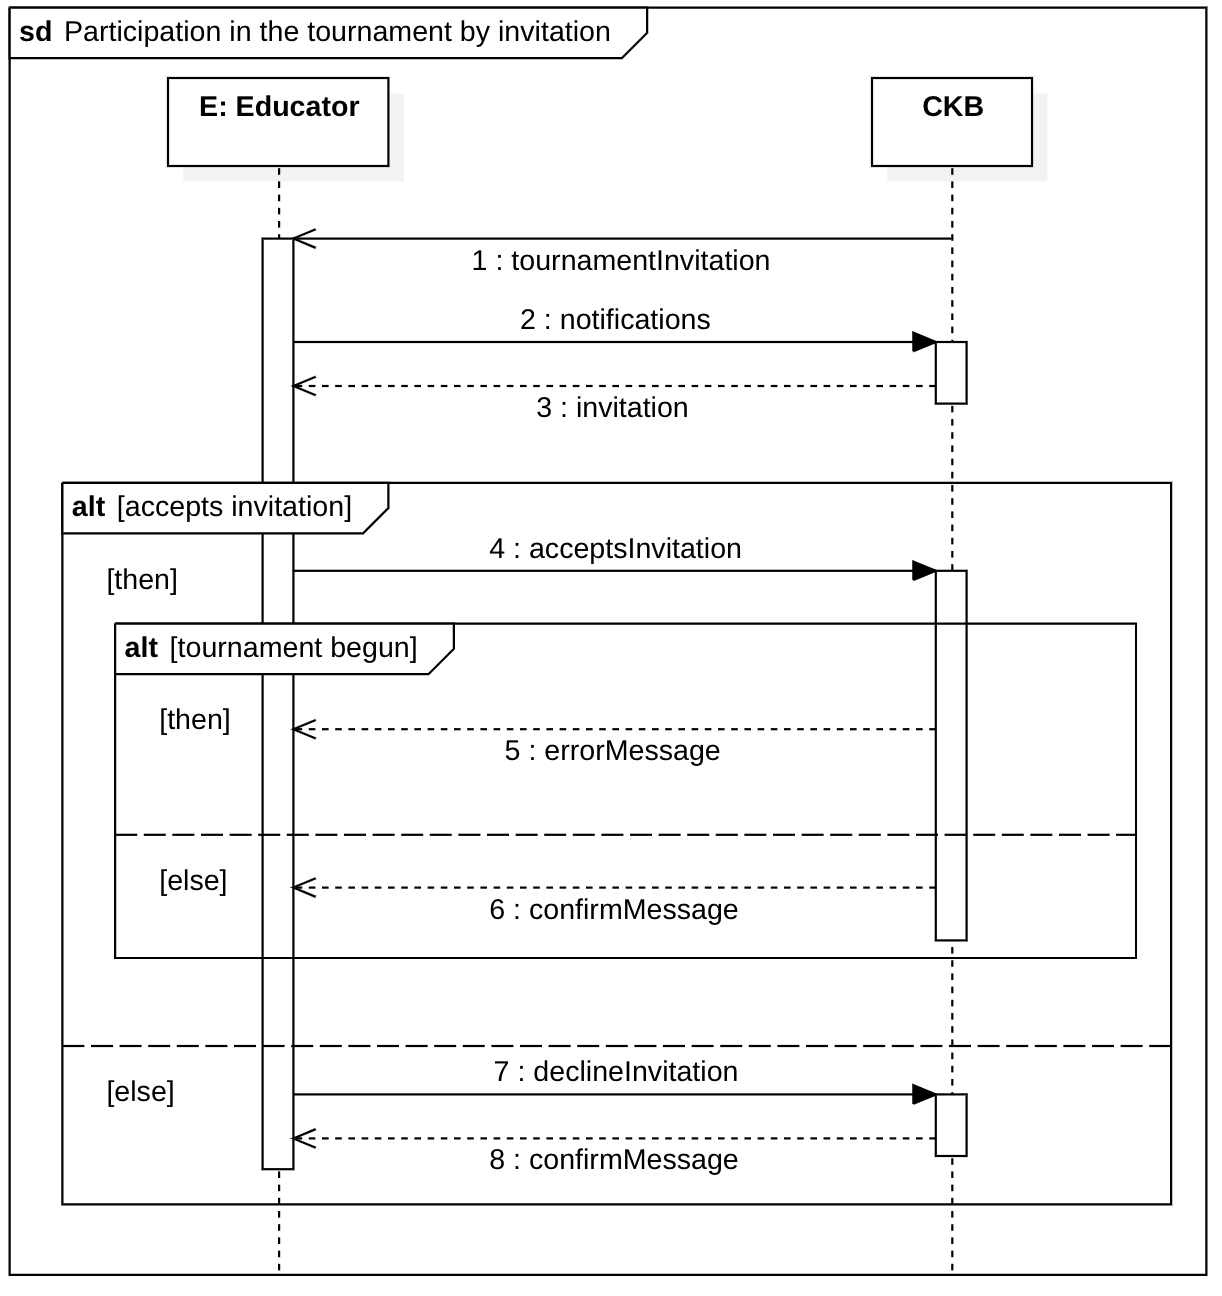
\includegraphics[scale=0.6]{images/SD/ParticipationTournamentInvitationSD.png} 
    \caption{Participation in a Tournament by invitation Sequence Diagram}
    \label{fig_SignUpTournamentSD}
\end{figure}




\subsubsection{Requirements mapping}

\renewcommand{\arraystretch}{1.5}
\vspace{1\baselineskip}

%GOAL 1
\begin{tabular}{|p{7.5cm}|p{7.5cm}|}
\hline
\multicolumn{2}{|p{15cm}|}{\textbf{[G1] Educator administers the tournaments and decides and manages the battles within them.}}\\

\hline
\vspace{2pt}&\vspace{2pt}\\
{[R3] The system allows the educator to register by entering firstname, lastname, email, password and username.}
&
{[D2] Educator must have an internet connection.}
\\

{[R4] The system allows registered educator to log in by entering username and password.}
&
{[D3] Educator be a very knowledgeable person in the area of software development.}
\\

{[R5]}The system allows the educator the ability to create of a tournament, allowing him or her to set a deadline for entries.
&
{[D8] Educator must make sure that the CodeKata he intends to upload, we have no errors inside.}
\\

{[R6] The system allows the educator to invite other educators to join the tournament.}
&
\\

{[R7] The system allows the educator who created the tournament, to close the tournament if all battles are completed.}
&
\\

{[R11] The system allows educators to see the list of all battles(unstarted, ongoing, and completed) in that tournament.}
& \\

{[R15] The system allows all members of the platform to see the list of ongoing tournaments.}
& \\

{[R16] The system allows all members of the platform to see the ranking of a tournaments, with the relative score associated with each student participating in the tournament.}
& \\

{[R17] The system sends a notification to educators who have been invited by the educator who created the tournament to participate in the creation of battles within the tournament.}
& \\

{[R18] System allows educators to accept or decline invitations to participate in the tournament.}
& \\
\vspace{2pt}&\vspace{2pt}\\
\hline
\end{tabular}
\clearpage
%continue
\begin{tabular}{|p{7.5cm}|p{7.5cm}|}
\hline
{[R19] The system allows all educators participating in the tournament to create battles by uploading the CodeKata and specifying the description, entry deadline, final project delivery deadline, minimum and maximum number of students in each team, if desired manual evaluation, and qualitative
aspects of the source to be evaluated.}
& \\

{[R20] The system when the battle is over allows the educator who created the battle to see each team’s final project.}
& \\

{[R21] The system allows the educator to evaluate each team’s final projects.}
& \\

{[R31] The system allows the battle educator to see the current ranking.}
& \\

{[R32] The system allows the battle educator to see the score of each team.}
& \\

{[R34] The system, at the end of the battle, allows educators participating in tournament to see the final ranking.}
& \\


\vspace{2pt}&\vspace{2pt}\\
\hline
\end{tabular}
\raggedright
\vspace{2\baselineskip}


%GOAL 2
\begin{tabular}{|p{7.5cm}|p{7.5cm}|}
\hline
\multicolumn{2}{|p{15cm}|}{\textbf{[G2] Students participate in tournaments by taking part in related battles, either individually or in groups.}}\\
\hline
\vspace{2pt}&\vspace{2pt}\\
{[R1] The system allows the student to register by entering firstname, lastname, email, password and username.}  
& 
{[D1] Student must have an internet connection.}
\\

{[R2] The system allows registered students to log in by entering username and password.}
&
{[D4] Student must have a GitHub account.}
\\

{[R8] The system allows students to register for the tournament by the deadline.}
&
{[D5] Students who are part of the team when they receive the main GitHub repository must fork it.}
\\

{[R9] The system allows student to unsubscribe from the tournament.}
&
{[D6] Students who are part of the team must set up an automated workflow through GitHub Actions to inform the platform.}
\\

{[R10] The system allows students enrolled in the tournament to see the list of all battles(unstarted, ongoing, and completed).}
&
{[D7] Students must have all the tools(e.g., IDE) to work on the project.}
\\

{[R12] The system notifies all students registered on the platform to inform them of the creation of a new tournament.}
&
{[D9] Students participating in a battle are expected to follow a test-first approach.}
\\

{[R14] The system when the educator closes the tournament, notifies all students in that tournament of the availability of the final ranking.}
&
\\

{[R15] The system allows all members of the platform to see the list of ongoing tournaments.}
& \\

{[R22] The system allows students registered for the tournament to see all the specifics of a battle.}
& \\

{[R23] The system allows students participating in the tournament to register for the battle by the deadline.}
& \\

\vspace{2pt}&\vspace{2pt}\\
\hline
\end{tabular}
%continua
\clearpage
\begin{tabular}{|p{7.5cm}|p{7.5cm}|}
\hline

{[R24] The system allows students participating in the battle to create teams by inviting other students participating in the same tournament.}
& \\

{[R25] The system when the battle enrollment expires must create the GitHub repository with the CodeKata in it.}
& \\

{[R26] The system when the battle enrollment expires sends the GitHub repository link to all members of each team and the instructions to fork the repository and set up an automated workflow.}
& \\

{[R29] The system allows students participating in the battle to see each team’s current score.}
& \\

{[R30] The system allows students participating in the battle to see the current ranking of the battle.}
& \\

{[R33] The system, at the end of the battle, allows students participating in tournament to see the final ranking.}
& \\

{[R35] The system, at the end of the battle, notifies all students participating in the battle of the availability of the final ranking.}
& \\

{[R36] The system sends a notification to all students participating in a tournament when a new battle is created.}
& \\

{[R37] The system sends a notification to students who have been invited by another student to join and form a team.}
& \\

{[R38] The system offers the possibility for students to accept or reject invitations received from other students to form a team.}
& \\

\vspace{2pt}&\vspace{2pt}\\
\hline
\end{tabular}
\raggedright
\vspace{2\baselineskip}

%GOAL 3
\begin{tabular}{|p{7.5cm}|p{7.5cm}|}
\hline
\multicolumn{2}{|p{15cm}|}{\textbf{[G3] The tournament implements a ranking derived from each student's individual score. This score is determined by aggregating the scores acquired by the student in each battle in which he took part.}}\\
\hline
\vspace{2pt}&\vspace{2pt}\\
{[R13] The system, at the end of each battle, updates each student’s score by summing the scores obtained in each completed battle in which he participated, reflecting these changes in the overall tournament ranking.}
& 
{[D1] Student must have an internet connection.}
\newline
{[D4] Student must have a GitHub account.}
\newline
{[D5] Students who are part of the team when they receive the main GitHub repository must fork it.}
\\

{[R25] The system when the battle enrollment expires must create the GitHub repository with the CodeKata in it.}
& 
{[D6] Students who are part of the team must set up an automated workflow through GitHub Actions to inform the platform.}
\\

{[R27] The system must retrieve the source from the team repository after each push by the team.}
& 
{[D7] Students must have all the tools(e.g., IDE) to work on the project.}
\\

{[R28] The system assigns a integer score from 0 to 100 to the project retrieved from the GitHub repository, according to the following aspects: functional aspects (number of test cases passed), timeliness (difference between the last team commit and the battle registration deadline), and source quality level, the latter evaluated by a third-party tool Sonarqube.}
& 
{[D9] Students participating in a battle are expected to follow a test-first approach.}
\\

\vspace{2pt}&\vspace{2pt}\\
\hline
\end{tabular}








\clearpage

\subsection{Performance Requirements}
\subsubsection{Number of Users}
In accordance with data published by other such applications, the CKB system expects to support about 20,000 users. So, we can consider that the system should be able to handle simultaneously the 50\% of them.

\subsubsection{Data Storage}
From the data storage point of view, the CKB system should consider several sources of data:
\begin{itemize}
    \item \textbf{Student's data}: about 19,000 students are expected
    \item \textbf{Educator's data}: about 1,000 educator are expected
    \item \textbf{Tournaments data}: 1,500 tournaments a year are expected
    \item \textbf{Battles data}: 12,000 battles a year are expected
\end{itemize}

\subsubsection{Time response}
CKB should ensure that the delay between an interaction with the system and its response should be no more than a couple of seconds, provided that the Internet connection is working correctly.


\subsection{Design Constraints}
\subsubsection{Standards compliance}
The system should respect all the laws regarding privacy and data treatment and exchange with third parties, to work in Europe, the system should respect the EU GDPR. In particular, a general description of the main principles that data should have in order to guarantee their privacy is given in Art. 5 of the GDPR document.

\subsubsection{Hardware limitations}
Following are all the hardware requirements:
\begin{itemize}
    \item An Internet connection that can be Wi-Fi, 2G/3G/4G/5G or Ethernet.
    \item And any electronic device that can connect to the internet and open a web browser. 
\end{itemize}

\subsubsection{Any other constraint}
There are not other constraints.

\subsection{Software System Attributes}

\subsubsection{Reliability}
With regard to reliability, since the system has no critical operations, the reliability rate can be about 1\%, which is in line with common standards. However, it is crucial to consider that the system also depends on third-party components over which no direct control is exercised. Despite this, it is critical to emphasize that any failure of such external components should not result in total system failure and loss of data.

\subsubsection{Availability}
Regarding the availability aspect, the platform can accept a level of 99\%. This implies that the system could be offline for a total period of 3.65 days per year. This choice is motivated by the fact that the platform does not provide critical or emergency services.
This decision reflects consideration of the non-critical nature of platform operations, allowing the system a limited period of downtime without significant impact on daily operations.

\subsubsection{Security}
The system handles sensitive personal data of users, emphasizing the crucial importance of security. The store must be subject to strict security measures to prevent any external or internal threats. Passwords inside are subjected to cryptographic processes. For communication through the Internet, the application uses an encryption protocol in order to avoid the possibility of eavesdropping and traffic manipulation (sniffing and spoofing). These precautions aim to ensure protection from fraudulent attacks, preserving user privacy and ensuring data integrity and consistency.

\subsubsection{Maintainability}
The system should be structured into distinct modules, each dedicated to specific functionality, with the goal of conforming to defined standards. This approach is intended to facilitate maintenance, replacement and, possibly, extension of modules, ensuring efficient management of the system over time. Each feature implemented must be thoroughly documented, providing clear and understandable details to facilitate understanding and management of the code. The combination of a modular structure, standards compliance, comprehensive documentation and a rigorous testing routine is critical to ensure effective management, maintainability and sustainable growth of the system over time.


\subsubsection{Portability}
The system is designed to operate on any web browser (e.g., Google Chrome, Safari, Firefox) in order to maximize its portability. This approach is intended to offer maximum versatility, allowing users to exploit the system across a wide range of web browsers.







